% Copyright (c) 2008-2009 solvethis
% Copyright (c) 2010-2016 Casper Ti. Vector
% Public domain.
%
% 使用前请先仔细阅读 pkuthss 和 biblatex-caspervector 的文档,
% 特别是其中的 FAQ 部分和用红色强调的部分。
% 两者可在终端/命令提示符中用
%   texdoc pkuthss
%   texdoc biblatex-caspervector
% 调出。

% 采用了自定义的(包括大小写不同于原文件的)字体文件名,
% 并改动 ctex.cfg 等配置文件的用户请自行加入 nofonts 选项;
% 其它用户不用加入 nofonts 选项,加入之后反而会产生错误。
\documentclass[UTF8]{pkuthss}

% 使用 biblatex 排版参考文献,并规定其格式(详见 biblatex-caspervector 的文档)。
% 这里按照英文文献在前,中文文献在后排序(“sorting = ecnty”);
% 若需按照中文文献在前,英文文献在后排序,请设置“sorting = centy”;
% 若需按照引用顺序排序,请设置“sorting = none”。
% 若需在排序中实现更复杂的需求,请参考 biblatex-caspervector 的文档。
\usepackage[backend = biber, style = caspervector, utf8, sorting = ecnty]{biblatex}

% 按学校要求设定参考文献列表中的条目之内及之间的距离。
\setlength{\bibitemsep}{3bp}
% 对于 linespread 值的计算过程有兴趣的同学可以参考 pkuthss.cls。
\renewcommand*{\bibfont}{\zihao{5}\linespread{1.27}\selectfont}

% 设定文档的基本信息。
\pkuthssinfo{
	cthesisname = {硕士研究生学位论文}, ethesisname = {Doctor Thesis},
	ctitle = {测试文档}, etitle = {Test Document},
	cauthor = {某某},
	eauthor = {Test},
	studentid = {0123456789},
	date = {某年某月},
	school = {某某学院},
	cmajor = {某某专业}, emajor = {Some Major},
	direction = {某某方向},
	cmentor = {某某教授}, ementor = {Prof.\ Somebody},
	ckeywords = {其一,其二}, ekeywords = {First, Second}
}
% 载入参考文献数据库(注意不要省略“.bib”)。
\addbibresource{thesis.bib}

% 普通用户可删除此段,并相应地删除 chap/*.tex 中的
% “\pkuthssffaq % 中文测试文字。”一行。
\usepackage{color}
% \def\pkuthssffaq{%
% 	\emph{\textcolor{red}{pkuthss 文档模版最常见问题:}}

% 	\texttt{\string\cite}、\texttt{\string\parencite} %
% 	和 \texttt{\string\supercite} 三个命令分别产生%
% 	未格式化的、带方括号的和上标且带方括号的引用标记:%
% 	\cite{test-en},\parencite{test-zh}、\supercite{test-en, test-zh}。

% 	若要避免章末空白页,请在调用 pkuthss 文档类时加入 \texttt{openany} 选项。

% 	如果编译时不出参考文献,
% 	请参考 \texttt{texdoc pkuthss}“问题及其解决”一章
% 	“上游宏包可能引起的问题”一节中关于 biber 的说明。
% }

\newcommand\todo[1]{\textcolor{red}{\{TODO:#1\}}}
\newcommand\mycode[1]{{\small\ttfamily #1}}
\usepackage{hyperref}

\usepackage{listings}
\lstset{
    numbers=left, 
    numberstyle=\tiny,
    keywordstyle= \color{ blue!70},
    commentstyle= \color{red!50!green!50!blue!50}, 
    frame=shadowbox, % 阴影效果
    rulesepcolor= \color{ red!20!green!20!blue!20},
    basicstyle=\small\ttfamily,
    breaklines
} 

\begin{document}
	% 以下为正文之前的部分,默认不进行章节编号。
	\frontmatter
	% 此后到下一 \pagestyle 命令之前不排版页眉或页脚。
	\pagestyle{empty}
	% 自动生成封面。
	\maketitle
	% 版权声明。封面要求单面打印,故需新开右页。
	\cleardoublepage
	% Copyright (c) 2008-2009 solvethis
% Copyright (c) 2010-2017 Casper Ti. Vector
% All rights reserved.
%
% Redistribution and use in source and binary forms, with or without
% modification, are permitted provided that the following conditions are
% met:
%
% * Redistributions of source code must retain the above copyright notice,
%   this list of conditions and the following disclaimer.
% * Redistributions in binary form must reproduce the above copyright
%   notice, this list of conditions and the following disclaimer in the
%   documentation and/or other materials provided with the distribution.
% * Neither the name of Peking University nor the names of its contributors
%   may be used to endorse or promote products derived from this software
%   without specific prior written permission.
%
% THIS SOFTWARE IS PROVIDED BY THE COPYRIGHT HOLDERS AND CONTRIBUTORS "AS
% IS" AND ANY EXPRESS OR IMPLIED WARRANTIES, INCLUDING, BUT NOT LIMITED TO,
% THE IMPLIED WARRANTIES OF MERCHANTABILITY AND FITNESS FOR A PARTICULAR
% PURPOSE ARE DISCLAIMED. IN NO EVENT SHALL THE COPYRIGHT HOLDER OR
% CONTRIBUTORS BE LIABLE FOR ANY DIRECT, INDIRECT, INCIDENTAL, SPECIAL,
% EXEMPLARY, OR CONSEQUENTIAL DAMAGES (INCLUDING, BUT NOT LIMITED TO,
% PROCUREMENT OF SUBSTITUTE GOODS OR SERVICES; LOSS OF USE, DATA, OR
% PROFITS; OR BUSINESS INTERRUPTION) HOWEVER CAUSED AND ON ANY THEORY OF
% LIABILITY, WHETHER IN CONTRACT, STRICT LIABILITY, OR TORT (INCLUDING
% NEGLIGENCE OR OTHERWISE) ARISING IN ANY WAY OUT OF THE USE OF THIS
% SOFTWARE, EVEN IF ADVISED OF THE POSSIBILITY OF SUCH DAMAGE.

% 此处不用 \specialchap,因为学校要求目录不包括其自己及其之前的内容。
\chapter*{版权声明}
% 综合学校的书面要求及 Word 模版来看,版权声明页不需加页眉、页脚。
\thispagestyle{empty}

任何收存和保管本论文各种版本的单位和个人,
未经本论文作者同意,不得将本论文转借他人,
亦不得随意复制、抄录、拍照或以任何方式传播。
否则一旦引起有碍作者著作权之问题,将可能承担法律责任。

% 若需排版二维码,请将二维码图片重命名为“barcode”,
% 转为合适的图片格式,并放在当前目录下,然后去掉下面 2 行的注释。
%\vfill\noindent
%\includegraphics[height = 5em]{barcode}

% vim:ts=4:sw=4


	% 此后到下一 \pagestyle 命令之前正常排版页眉和页脚。
	\cleardoublepage
	\pagestyle{plain}
	% 重置页码计数器,用大写罗马数字排版此部分页码。
	\setcounter{page}{0}
	\pagenumbering{Roman}
	% 中英文摘要。
	% Copyright (c) 2014,2016 Casper Ti. Vector
% Public domain.

\begin{cabstract}

程序调试是一个耗费时间的任务,已经有很多研究者提出了各种不同的自动缺陷定位技术去减轻手动调试的负担。
在这些自动缺陷定位技术中,基于频谱的缺陷定位和基于状态覆盖的缺陷定位是两种比较常用的缺陷定位技术。
这两种技术都是在执行时收集一些统计信息。
这两种技术存在一些相似之处,但是两种技术一直单独地发展,而它们的结合也一直没有被系统地讨论过。

本文对基于频谱的缺陷定位和基于状态覆盖的缺陷定位技术的结合进行了系统的实证研究,
并且提出一种基于机器学习的谓词预测的方法帮助缺陷定位。
本文构建了一个两种技术的统一模型,并在这个模型上系统地探索了四种变体:
不同粒度的数据收集、不同的怀疑度公式、不同的怀疑度结合方式、不同的谓词。
此外,本文还提出了一个基于机器学习的谓词预测模型,来完善基于状态覆盖的缺陷定位原有的预定义谓词。

本文的研究得到了很多结论。
第一,更细粒度的数据收集的效果远远好于粗粒度的数据收集,并且只需要花费稍微多一点的执行时间。
第二,把基于频谱的缺陷定位公式应用在基于状态覆盖的缺陷定位的预定义谓词上,其效果反而好于原有的基于状态覆盖的缺陷定位的公式。
第三,一个基于频谱的缺陷定位和基于状态覆盖的缺陷定位的线性结合模型的效果比两者都更好。
第四,结合方法的效果大部分得益于分支谓词。
第五,预测的谓词在某些指标上获得了比预定义谓词更好的结果。预测谓词与预定义谓词具有互补性,两者结合后定位效果进一步提升。

\end{cabstract}

\begin{eabstract}

Program debugging is a time-consuming task,
and researchers have proposed different kinds of automatic fault localization techniques
to mitigate the burden of manual debugging.
Among these techniques, two popular families are spectrum-based fault localization
and statistical debugging,
both localizing faults by collecting statistical information at runtime.
Though the ideas are similar, the two families have been developed independently
and their combinations have not been systematically explored.

In this paper we perform a systematical empirical study on the combination of spectrum-based
fault localization and statistical debugging,
and we propose a predicate prediction technique based on machine learning to help to locate the faults.
We first build a unified model of the two techniques,
and systematically explores four types of variations:
different granularities of data collection,
different risk evaluation formulas, different ways of combining suspiciousness scores,
and different predicates.
Then we propose a machine-learning model to predict the predicates,
instead of using pre-defined predicates in statistical debugging.

The study leads to several findings.
First, fine-grained data collection significantly outperforms
coarse-grained data collection with a little more execution overhead.
Second, the risk evaluation formulas of spectrum-based fault localization
siginificantly outperforms that of statistical debugging when used in statistical debugging.
Third, a linear combination of spectrum-based fault localization and
statistical debugging outperforms both individual approaches.
Forth, most of the effectiveness of the combined approach contributed by a simple type of predicates:
branch conditions.
Fifth, the predicted predicates are better than pre-defined predicates in some metrics.
The predicated predicates and pre-defined predicates are complementary.
The combination of them has further improvement.
\end{eabstract}

% vim:ts=4:sw=4

	% 自动生成目录。
	\tableofcontents

	% 以下为正文部分,默认要进行章节编号。
	\mainmatter
	% 各章节。
	\chapter{引言}

本章主要介绍了自动缺陷定位的研究背景及其重要意义,然后阐述了本文的研究内容、主要贡献和论文结构。

\section{研究背景}

随着软件的发展,生活中越来越多的方面都与软件有着紧密的关系。
小到人们的日常出行、购物、餐饮等,大到航空航天、医药等领域,软件在人们的生活中扮演着重要的角色。
随着软件的应用领域的扩大,软件的复杂性上升,提升了软件缺陷的可能性。
软件缺陷可能会导致巨大的损失。
一个著名的被广泛引用的例子是海湾战争时,一颗导弹由于导航软件的精度缺陷而偏离了目标,导致28人死亡和100人受伤\parencite{Zou2015A}。
2002年,美国国家标准与技术研究院(NIST)发表的一篇报告\parencite{NIST2002The}显示,软件缺陷每年会导致约595亿美元的经济损失。
发现并修复软件缺陷,保障软件的高质量成为一项重要的任务。

\section{研究意义}

在发现软件缺陷之后,开发人员为了解决这个缺陷往往需要三步\parencite{Parnin2011Are}。
第一步,缺陷定位,需要找到程序中和这个缺陷有关的语句。
第二步,理解缺陷,明白为什么会发生缺陷。
第三步,修复缺陷,修改代码以让缺陷消失。
这三个步骤合起来就是调试的过程。缺陷定位作为调试的第一步,其完成速度和准确性对后面的步骤有着很大的影响。
在传统的开发环境当中,人们可以手动调试来定位缺陷,比如插入断点、打印日志信息等等。
在1989年Collofello等人就指出尝试去减少软件中的错误会花费50\%到80\%的开发和维护的精力\parencite{Collofello1989Evaluating}。
随着软件的复杂性的上升,手动地定位软件缺陷将会耗费更多开发者的时间和精力。
为了提高定位缺陷的速度,研究人员对自动化的缺陷定位展开了研究,并取得了巨大的进展
\parencite{Weiser1981Program,Weiser1984Program,Reps1997The,Ball2003From,Groce2004Understanding,
Jones2002Visualization,Liblit2005Scalable,Liu2005SOBER,
Renieres2003Fault,Abreu2006An,Xie2013A,W2009BP,
Wong2012Effective,Le2016A,Papadakis2015Metallaxis,Moon2014Ask,Zhang2006Locating,
Chandra2011Angelic,Shapiro1982Algorithmic,Zeller2002Isolating,Zeller2002Simplifying}。
然而在2011年,Partin和Osro的一篇调查\parencite{Parnin2011Are}通过研究缺陷定位技术在实际应用场景下的效果,发现以往的评价指标并不能准确的反映缺陷定位技术在实际应用中的效果。
以往的缺陷定位技术是基于一系列关于开发人员会如何调试的假设,而这些假设在实际场景的某些情况下会失效。
自动化缺陷定位技术还有很大的发展空间。

\section{本文研究内容和主要贡献}

为了能提升调试的效率,本文对自动化缺陷定位技术进行了深入的研究。
通过在实际缺陷中分析传统的缺陷定位技术的效果,本文提出了一种结合基于频谱的缺陷定位和基于状态覆盖的缺陷定位的方式。
本文探索了各种不同的结合方式的效果,分析了基于状态覆盖的缺陷定位公式的不足,并使用基于频谱的缺陷定位公式与其互补。
同时,由于基于状态覆盖的缺陷定位使用的预定义谓词的不灵活性,
本文提出了一种基于机器学习的谓词预测模型,而传统的基于状态覆盖的缺陷定位使用的是预定义谓词。
预测出的谓词与预定义谓词互补,能进一步提升定位效果。

本文的贡献如下:
\begin{itemize}
\item 在实际缺陷中深入分析了基于频谱的缺陷定位的效果,发现了基于频谱的缺陷定位利用的频谱信息粒度不够细,导致缺陷和非缺陷无法区别。
\item 在实际缺陷中深入分析了基于状态覆盖的缺陷定位的效果,发现了其怀疑度公式在实际缺陷中并不适用。
\item 提出了结合基于频谱的缺陷定位和基于状态覆盖的缺陷定位的方式。基于状态覆盖的缺陷定位的信息粒度比基于频谱的缺陷定位的信息粒度细,
而基于频谱的缺陷定位公式在实际缺陷中仍然表现良好,两者结合之后获得了更好的效果。
\item 利用结合后的模型,在实际缺陷中分析了基于状态覆盖的缺陷定位的谓词起作用的原因,发现分支是起最大作用的谓词。
\item 提出了一种基于机器学习的预测谓词的模型,能够根据语句上下文预测谓词,从而更好地定位缺陷。
\end{itemize}

\section{论文结构}

本文共七章,结构如下:

第一章为引言,介绍了本文的研究背景、研究意义、研究内容和主要贡献。

第二章为相关工作,介绍了国内外相关领域的研究现状,包括自动缺陷定位技术、机器学习技术和实验数据集三部分。

第三章为问题分析,在实际缺陷中分析了现有自动缺陷定位技术的优势和不足。

第四章介绍了基于谓词预测的结合现有技术的缺陷定位工具的设计,包括结合现有技术的方法、基于机器学习的谓词预测模型等等。

第五章介绍了基于谓词预测的结合现有技术的缺陷定位工具的实现,包括整个代码流程和各个模块的实现方式。

第六章是本文提出的缺陷定位工具的实验与验证。

第七章是对全文的总结和对未来工作的展望。


	\chapter{相关工作}

本章将介绍自动缺陷定位、机器学习的相关工作和缺陷定位所使用的数据集以帮助更好理解本文的工作。

\section{自动缺陷定位相关工作}

程序切片\parencite{Weiser1981Program,Weiser1984Program}是自动调试最早的技术之一,
但是程序切片之后可能出错的语句数量仍然比较庞大。
为了解决程序切片调试方法的短板,一种通过观察错误程序的执行特征和正确程序的执行特征的调试技术被提出。
这些技术通过收集程序执行信息,观察不同的某种特征,来定位缺陷。
比如使用路径概要\parencite{Reps1997The},反例\parencite{Ball2003From,Groce2004Understanding},语句覆盖\parencite{Jones2002Visualization}和谓词值\parencite{Liblit2005Scalable,Liu2005SOBER}等等。

本文根据北京大学熊英飞研究员对缺陷定位的分类\parencite{YingfeiFL},将缺陷定位分为以下几类。

\begin{itemize}
\item 基于切片的缺陷定位
\item 基于频谱的缺陷定位
\item 基于状态覆盖的缺陷定位
\item 基于变异的缺陷定位
\item 基于构造正确执行状态的缺陷定位
\item 基于算法式调试的缺陷定位
\item 基于差异化调试的缺陷定位
\end{itemize}

本文的研究内容主要根据基于频谱的缺陷定位和基于状态覆盖的缺陷定位。

\subsection{基于切片的缺陷定位}

Weiser在1981年提出的程序切片\parencite{Weiser1981Program,Weiser1984Program}是自动调试(特别是缺陷定位)最早的技术之一。
给定一个程序$P$和一个在$P$的语句$s$中使用的变量$v$,程序切片会找到$P$中所有可能会影响$s$中$v$的值的语句。
如果$s$中$v$的值是错误的,那么导致这个错误的缺陷语句一定在这个切片当中。
也就是说,不在这个切片当中的语句可以在调试过程中被忽略。
尽管程序切片已经减少了可能出错的语句的数量,但是切片中的语句的数量仍然比较大。
为了解决这个问题,Korel和Laski在1988年提出了动态程序切片\parencite{Korel1988Dynamic}。
动态程序切片计算某一个特定执行的切片。
后来又有很多的动态程序切片的变种被提出\parencite{Demillo1996Critical,Gyim1999An,Zhang2006Pruning,Zhang2003Precise},用于解决调试问题,并且产生了大量研究工作\parencite{Agrawal1993Debugging,Liu2007Indexing,Al2005The,Alves2011Fault,Ju2014HSFal,Wotawa2010Fault,Mao2014Slice}。

\subsection{基于频谱的缺陷定位}

基于频谱的缺陷定位是使用最广泛的自动化缺陷定位方法\parencite{YingfeiFL}。
程序频谱(~Program~ Spectrum)最早由Reps等人于1997年提出\parencite{Reps1997The},用于解决千年虫问题。
Harrold 等人在2002年\parencite{Harrold2000An}提出使用测试覆盖信息作为频谱信息的调试方法。
Renieris等人在 2003年提出使用通过的测试用例和失败的测试用例进行缺陷定位\parencite{Renieres2003Fault},奠定了此后基于频谱的缺陷定位的基础。

考虑一种极端的情况。
比如当某一个语句$s$被执行的之后,测试用例就会失败。
而通过的测试用例都不会执行语句$s$。
那么语句$s$很有可能就是导致缺陷的语句。
找出所有这样的语句$s$就可以大幅减少需要排查错误的语句。
但是,在实际的代码中这种极端的情况很少出现。
对于一个出错的语句$s$,它很可能既被失败的测试用例执行,也被通过的测试用例执行。
因为一个语句在其不同的上下文作用下会产生不同的效果。
简单地计算通过的测试用例覆盖的语句和失败的测试用例覆盖的语句的差集是无法准确找出错误语句的。
利用通过的测试用例覆盖的语句的交集和并集,与失败的测试用例覆盖的语句取差集,是最早的一种基于频谱的缺陷定位方法\parencite{Renieres2003Fault}。
这种方法也隐含着基于频谱的缺陷定位的假设:被失败的测试用例执行的语句,更有可能有错误。而被通过的测试用例执行的语句,更有可能是正确的。

Jones等人提出的Tarantula\parencite{Jones2002Visualization},直观地给开发者展示了每个语句在通过的测试用例和失败的测试用例下的参与情况。
参与情况也被称为怀疑度。
% 每条语句的参与情况,使用公式
% $$
% \mathrm{Tarantula}(s) = \frac{\frac{a_{ep}}{a_{p}}}{\frac{a_{ep}}{a_{p}} + \frac{a_{ef}}{a_{f}}}
% $$
% 计算。
% 这个公式计算的值也被称为怀疑度。
怀疑度更高的语句会在怀疑列表更靠前的位置。
相比于交集并集差集的方法,Tarantula在Siemens数据集上可以将错误的语句放在怀疑列表更前面的位置\parencite{Jones2005Empirical}。

Tarantula之后,又有很多计算怀疑度的公式被提出。
效果比较好的Ochiai由Abreu等人提出\parencite{Abreu2006An}。
% $$
% \mathrm{Ochiai}(s) = \frac{a_{ef}}{\sqrt{a_{f} \times (a_{ef} + a_{ep})}}
% $$
Ochiai由\parencite{Meyer2004Comparison}提出用于计算基因的相似度。
Abreu等人将其引入用于计算怀疑度,并与Jaccard\parencite{Chen2002Pinpoint},Tarantula,AMPLE\parencite{Dallmeier2005Lightweight}比较,发现Ochiai计算的怀疑度使得定位效果更好\parencite{Abreu2006An,Abreu2007On}。
此后Xie等人在理论上证明了不存在单一最佳公式\parencite{Xie2013A},
对怀疑度公式的研究一直没有停下。

除了直接提出用于计算的公式之外,研究人员也开始使用机器学习的方法去学习怀疑度的公式。
Wong等人提出使用反向传播神经网络来定位缺陷\parencite{W2009BP}。
使用的输入数据是频谱信息(语句覆盖信息)和对应的测试用例是通过还是失败。
输入数据每一行对应一个测试用例。
第i列为1表示的是该测试用例覆盖了第i个语句,为0则表示没有覆盖。
预测的标签为1表示该测试用例失败了,为0表示通过了。
为了减少需要分析的可能出错的语句的个数(每一行输入数据的维度),优先使用所有失败的测试用例覆盖的语句。
此后Wong又提出了使用径向基核函数的神经网络来定位缺陷\parencite{Wong2012Effective}。

\subsection{基于状态覆盖的缺陷定位}

在缺陷定位的时候,定位的程序元素的大小也会影响结果。程序元素可以是一条语句,一个方法,一个文件。
程序元素的粒度越细,对测试信息的利用越精确。
然而单个元素上覆盖的测试数量越少,统计显著性越低。
如果把程序的每个执行状态作为程序元素,那么这会是一个比语句更加精细的粒度。
定位结果也将更加精细,对测试的利用也会更加充分。
但是,几乎不会有两个测试覆盖完全相同的状态,因为一个状态所包含的上下文信息往往十分复杂,很难完全一致。
于是使用抽象状态代替具体状态。
使用谓词将具体状态划分为抽象状态。
谓词是形如\mycode{a $>$ 0}这样的条件表达式。

Liblit等人最早提出了预定义谓词来划分状态\parencite{Liblit2005Scalable},并提出了统计性调试。
通过预定义在哪些代码结构中插入哪些谓词,统计性调试能够收集到许多抽象状态的覆盖情况。
% 利用表\ref{state_symbol}中的数学符号,统计性调试的公式可以表达为
% $$
% \mathrm{StatisticalDebugging}(s) = \frac{2}{\frac{1}{\frac{t_f}{t_f + t_p} - \frac{a_f}{a_f + a_p}} + \frac{log(F)}{log(t_f)}}
% $$

Liu等人改进了计算公式,提出了SOBER\parencite{Liu2006Statistical}。
虽然Liblit的方法可以有效定位一些错误,但是Liblit的方法只考虑了一个谓词是否在一次执行中为真,
而没有考虑为真的次数。
SOBER提出新的计算公式,从概率分布的角度来计算怀疑度。
% 公式计算的是对一个谓词,在失败的测试用例下这个谓词为真的概率分布,和在通过的测试用例下这个谓词为真的概率分布是否相似。
% 如果概率分布无论是在失败的测试用例中还是通过的测试用例中都一样,那么这个谓词对应的变量等和缺陷的关系就越小。
% 如果两个概率分布相差很大,说明这个谓词对应的抽象状态很有可能就有缺陷状态。
% 引入这个缺陷状态的语句很可能就是出错的语句。

除了预定义谓词以外,研究人员还提出各种从程序中获取谓词的方法。
Le等人提出 Savant\parencite{Le2016A} ,使用程序中的不变式的变化来划分状态。
程序中的不变式使用 Daikon\parencite{Ernst2007The} 挖掘。
Savant使用Learning-to-rank方法,通过分析经典的怀疑度分数和在通过的测试用例和失败的测试用例上观察到的不变式,来定位错误的方法。
Savant基于三个出发点。一,在失败的测试用例和通过的测试用例中表现出不同的不变式的程序元素,被怀疑是有错误的。
二,如果这些程序元素拥有很高的经典的怀疑度分数,那么它们更有可能是错误的。
三,有一些不变式比其他不变式更加可疑,比如\mycode{ x == null}。
% 而 Savant 的工作并没有引用 Liblit \parencite{Liblit2005Scalable}和 Liu \parencite{Liu2006Statistical},
% 很可能是在不知道统计性调试的情况下完成的。

\subsection{基于变异的缺陷定位}

变异是对程序的任意随机修改,由变异算子得到。
变异分析是测试领域的一个概念,被用于衡量一个测试集的好坏。
变异分析在程序中插入变异,得到很多变异体,然后使用一组测试去执行变异体。
如果一个测试集中任意测试在一个变异体上得到不同的结果,那么这个变异体被这个测试杀死。
能杀死越多变异体的测试集越好。

变异被引入缺陷定位,用于定位缺陷。
Papadakis等人提出Metallaxis\parencite{Papadakis2015Metallaxis},一个基于变异的缺陷定位。
Metallaxis基于两个假设:
\begin{itemize}
\item 当变异和错误在一个程序的同一条语句上时,失败的测试用例输出发生变化的概率大于通过的测试用例输出发生变化的概率。
\item 当变异和错误不在同一条语句上时,通过测试用例输出发生变化的概率大于失败的测试用例输出发生变化的概率。
\end{itemize}
基于表\ref{mutant_symbol},Metallaxis的怀疑度计算公式为
$$
\mathrm{Metallaxis}(m) = \frac{m_f}{\sqrt{F \times (m_f + m_p)}}
$$
与Ochiai类似。

Moon等人提出另一个基于变异的缺陷定位技术MUSE\parencite{Moon2014Ask}。
MUSE利用变异分析去捕捉单个语句和观察到的缺陷之间的关系。
MUSE基于的两个假设是:
\begin{itemize}
\item 一个失败的测试用例,比起在变异了正确语句的变异体上,在变异了错误语句的变异体上更容易变成通过的。
\item 一个通过的测试用例,比起在变异了失败语句的变异体上,在变异了正确语句的变异体上更容易变成失败的。
\end{itemize}
基于表\ref{mutant_symbol},MUSE的怀疑度计算公式为
$$
\mathrm{MUSE}(m) = m_{f2p} - m_{p2f} \times \frac{\sum_{m}^{}{m_{f2p}}}{\sum_{m}^{}{m_{p2f}}}
$$

\begin{table}
\centering
\caption{基于变异的缺陷定位的数学符号及其意义}
\begin{tabular}{|c|c|}
\hline
$m$ & 变异体 \\
\hline
$m_f$ & 变异m导致输出发生变化的失败的测试用例个数 \\
\hline
$m_p$ & 变异m导致输出发生变化的通过的测试用例个数 \\
\hline
$m_{f2p}$ & 变异m导致失败的测试用例变成通过的测试用例的个数 \\
\hline
$m_{p2f}$ & 变异m导致通过的测试用例变成失败的测试用例的个数 \\
\hline
$F$ & 失败的测试用例的个数 \\
\hline
\end{tabular}
\label{mutant_symbol}
\end{table}

\subsection{基于构造正确执行状态的缺陷定位}

MUSE通过变异体,可以把失败的测试用例变成通过,通过的测试用例变成失败的。
假如有一个变异体,它可以把失败的测试用例变成通过的,且不会影响通过的测试用例,那么这个变异体很可能就是缺陷的补丁。
但是直接分析出这样的变异体是很困难的。

Zhang提出的谓词翻转\parencite{Zhang2006Locating}巧妙地避免了直接分析出正确的补丁,而是使用改变程序状态来达到相同的目的。
假如出错的是一个布尔表达式,改变程序中一个布尔表达式的取值(把真变成假,或者把假变成真),强制改变执行的分支。
假如谓词翻转后,失败的测试用例变成通过的,那么对应的布尔表达式很可能有错误。

谓词翻转是局限在布尔表达式,天使调试\parencite{Chandra2011Angelic}则试图解决任意表达式的错误。
天使调试要求同时具有天使性和灵活性。
天使性是指,存在常量c(天使值)把表达式的求值结果替换成c,失败的测试变得通过。
灵活性是指,对于一个修复的候选$e$,和一个通过测试用例输入$I_p$,如果把$e$
的值替换成一个不同的值(不同于$I_p$下$e$的值),这个测试仍然通过。
利用符号执行约束求解计算得到天使值。
也由于符号执行的开销,天使调试无法应用到大型程序上。

\subsection{基于算法式调试的缺陷定位}

Shapiro提出的算法式调试\parencite{Shapiro1982Algorithmic},通过对子问题询问“是”或“否”来定位缺陷。
算法式调试把复杂的计算步骤拆为小的子问题。
算法式调试的一个问题是,子问题的正确结果可能是不知道的。
如果是让人进行交互式地判断,那么人需要花费时间计算判断子问题的结果。

\subsection{基于差异化调试的缺陷定位}

差异化调试由Zeller等人提出\parencite{Zeller2002Isolating,Zeller2002Simplifying}。
不同于以往的使用动态分析或静态分析的方法去关注源代码,
差异化调试关注程序状态,特别地,差异化调试关注当程序没有出错时的程序状态和程序出错时的程序状态。
差异化调试尝试找到一个最小的修改集合,当把这个集合应用到没有出错时的程序状态后,程序出错了。

\section{机器学习相关工作}

近年来,机器学习相关的工作在高速地发展中。
机器学习也越来越多地被应用到软件工程的领域,并且发挥着重要的作用。
神经网络是一种常用的机器学习模型。
神经网络的定义多种多样,采用 Kohonen 1998年在期刊《Neural Networks》上的定义,为
“神经网络是由具有适应性的简单单元组成的广泛并行互连的网络,它的组织能够模拟生物神经系统对真是世界物体所作出的交互反应”。
本文使用的误差后向传播网络能够近似复杂的非线性函数\parencite{Hecht1992Theory}。
Neumann等人提出一种结合了主成分分析和误差后向传播网络的软件风险分析\parencite{Neumann2002An}。
Tadayon使用神经网络做软件代价评估。
在缺陷定位方面,也有很多神经网络的应用。
比如之前提到的Wong的两篇工作\parencite{W2009BP,Wong2012Effective}。

\section{缺陷定位的数据集}

要研究缺陷定位,需要一个包含缺陷的数据集。
这个数据集一般来说需要有多个缺陷。
对每一个缺陷,会有对应的测试用例,和对应的一个正确的版本。
这些测试用例中既有通过的,也必定有失败的。
失败的这个测试用例就是由缺陷导致。

Siemens数据集\parencite{Hutchins1994Experiments}是一个很早的数据集,用于测试充分性的实验。
它由七个C程序组成,大小在141行到512行之间。
这七个C程序衍生出132个有缺陷的C程序。
每一个错误版本会恰好有一个缺陷。
这个缺陷可能涉及多行甚至多个文件。
但是这些程序的缺陷是由作者手动插入的,根据作者的描述其实和一个简单的变异操作非常相似。
Siemens数据集的输入被构造用于实现完全的代码覆盖。
尽管它一开始并不是被用于缺陷定位,但是很多缺陷定位技术都使用它来验证效果,比如最早的基于频谱的缺陷定位方法\parencite{Renieres2003Fault},Ochiai\parencite{Abreu2006An,Abreu2007On},
SOBER\parencite{Liu2006Statistical},BPNN\parencite{W2009BP}等等。

Defects4j数据集\parencite{Just2014Defects4J}是一个真实、独立、可重现缺陷的数据集。
它的v1.0版本由五个Java开源项目的357个缺陷组成(该数据集仍在更新当中)。
每一个错误版本会恰好有一个缺陷。
这个缺陷可能涉及多行甚至多个文件。
与Siemens数据集相比,~Defects4j~数据集的缺陷和测试用例都更接近实际开发情况。
Savant\parencite{Le2016A}就是在Defects4j数据集上验证的。

	\chapter{问题分析}

本章将基于频谱的缺陷定位和基于状态覆盖的缺陷定位应用在数据集Defects4j的某些缺陷上,
分析这些技术在实际缺陷上的优点与不足。

\section{使用基于频谱的缺陷定位}

基于频谱的缺陷定位对代码的内容没有假设,所使用的信息只有语句的覆盖情况。
考虑Defects4j中math项目的第五个缺陷,其代码如下:
\lstset{language=Java}
\begin{lstlisting}
public Complex reciprocal() {
    if (isNaN) {
        return NaN;
    }

    if (real == 0.0 && imaginary == 0.0) {
        return NaN; // Faulty code
                    // Should be "return INF;"
    }
    ...
}
\end{lstlisting}

为了使用基于频谱的缺陷定位,我们运行测试用例,并且收集语句的覆盖情况。
针对第2,3,6,7行语句,得到语句的覆盖情况如表\ref{math_5_statecover}所示。共有一个失败的测试用例。

\begin{table}
\centering
\begin{tabular}{|c|c|c|}
\hline
语句 & 被覆盖的失败测试用例个数 & 被覆盖的通过测试用例个数 \\
\hline
2 & 1 & 5 \\
3 & 0 & 1 \\
6 & 1 & 4 \\
7 & 1 & 0 \\
\hline
\end{tabular}
\caption{Defects4j中Math的第五个缺陷的测试用例覆盖语句的情况}
\label{math_5_statecover}
\end{table}

可以发现,第3行肯定不是缺陷语句,因为它没有被失败的测试用例覆盖过。
第2,6,7行都有可能是缺陷语句。
这三行都是被一个失败测试用例覆盖。
根据它们被覆盖的通过测试用例的个数,可以知道第7行最有可能出错,其次是第6行,最后是第2行。
这是根据了基于频谱的缺陷定位的假设,即被失败的测试用例执行的语句,更有可能有错误。而被通过的测试用例执行的语句,更有可能是正确的。

为方便此后的表述,引入一些数学符号,见表\ref{spec_symbol}。表中的统计量就是程序频谱。
\begin{table}
\centering
\begin{tabular}{|c|c|}
\hline
$a_{ef}$ & 一个语句被失败的测试用例覆盖的次数 \\
\hline
$a_{nf}$ & 一个语句未被失败的测试用例覆盖的次数 \\
\hline
$a_{ep}$ & 一个语句被通过的测试用例覆盖的次数 \\
\hline
$a_{np}$ & 一个语句未被通过的测试用例覆盖的次数 \\
\hline
$a_{f}$ & 失败的测试用例的个数 \\
\hline
$a_{p}$ & 通过的测试用例执行的次数 \\
\hline
\end{tabular}
\caption{基于频谱的错误定位的数学符号及其意义}
\label{spec_symbol}
\end{table}

表\ref{susp_formula}中列出了部分经典的怀疑度公式。
这些公式都遵循被失败的测试用例执行的语句,更有可能有错误。而被通过的测试用例执行的语句,更有可能是正确的。

\begin{table}
\centering
\begin{tabular}{|c|c|c|}
\hline
公式名称 & 公式 \\
\hline
Ochiai\parencite{Abreu2006An} & $\mathrm{Susp}(s) = \frac{a_{ef}}{\sqrt{a_{f} \times (a_{ef} + a_{ep})}}$ \\
\hline
Tarantula\parencite{Jones2002Visualization} &
$\mathrm{Susp}(s) = \frac{\frac{a_{ep}}{a_{p}}}{\frac{a_{ep}}{a_{p}} + \frac{a_{ef}}{a_{f}}}$ \\
\hline
Barinel\parencite{Abreu2009Spectrum} &
$\mathrm{Susp}(s) = 1 - \frac{a_{ep}}{a_{ep} + a_{ef}}$ \\
\hline
DStar\parencite{Wong2014The} &
$\mathrm{Susp}(s) = \frac{2}{a_{ep} + (a_f - a_{ef})}$ \\
\hline
Op2\parencite{Naish2011A} &
$\mathrm{Susp}(s) = a_{ef} - \frac{a_{ep}}{a_p + 1}$ \\
\hline
\end{tabular}
\caption{部分基于频谱的缺陷定位怀疑度公式}
\label{susp_formula}
\end{table}

利用表\ref{susp_formula}中的公式,计算第2,6,7行的怀疑度,得到表\ref{math_5_susp}。
可以发现,这五个怀疑度公式都满足
$$
\mathrm{Susp}(7) > \mathrm{Susp}(6) > \mathrm{Susp}(2)
$$
这五个怀疑度公式都认为第7行是最有可能出错的语句,而第7行也确实是出错的语句。
这些公式之间的差距不同。比如Tarantula和Op2认为这三行的怀疑度是非常接近的。
Ochiai,Barinel和DStar认为第2行和第6行的怀疑度接近,而第7行的怀疑度明显高于第2行和第6行的怀疑度。

这个例子体现了基于频谱的缺陷定位准确定位错误的能力。
但是实际上效果往往没有这么好。
其实在该缺陷中,还存在一个正确的语句,它被一个失败的测试用例覆盖过,且从没有被正确的测试用例覆盖过。
这个正确的语句的频谱信息和错误语句的频谱信息完全一致,所以它们的分数会相同。
而这个正确的语句将会干扰开发者对缺陷的分析。

\begin{table}
\centering
\begin{tabular}{|l|c|c|c|}
\hline
公式 & 第2行 & 第6行 & 第7行 \\
\hline
Ochiai & 0.4082 & 0.4472 & 1.0000 \\
\hline
Tarantula & 0.9988 & 0.9990 & 1.0 \\
\hline
Barinel & 0.1667 & 0.2000 & 1.0 \\
\hline
DStar & 0.2000 & 0.2500 & Infinity \\
\hline
Op2 & 0.9988 & 0.9990 & 1.0 \\
\hline
\end{tabular}
\caption{Defects4j中Math的第五个缺陷的经典公式怀疑度}
\label{math_5_susp}
\end{table}

\section{使用基于状态覆盖的缺陷定位}
\label{sec:state_based}

考虑Defects4j数据集中Math的第二个缺陷,其代码如下:
\lstset{language=Java}
\begin{lstlisting}
public double getNumericalMean() {
    return (double) (getSampleSize() * getNumberOfSuccesses()) / (double) getPopulationSize(); // Faulty code
    // Should be "return getSampleSize() * (getNumberOfSuccesses() / (double) getPopulationSize())"
}
\end{lstlisting}

使用Ochiai方法的话,该错误语句被排到第11位。
并列的分数将取其平均排名(期望排名),这是很多研究方法所使用的评估方式\parencite{Pearson2017Evaluating,Xuan2014Learning,Steimann2013Threats,Wong2016A}。
事实上该语句的分数位列第2位,但是一共有17个语句和该语句分数并列,导致最终排名为第11位。
基于频谱的缺陷定位方法在这里失效了,因为获取的信息不足。
其实这个缺陷更加适合使用基于状态覆盖的缺陷定位技术。

状态覆盖就是使用谓词把具体状态划分为抽象状态。
比如,对于如下代码,
\lstset{language=Java}
\begin{lstlisting}
a = Math.abs(a);
if (update_b) {
    b = Math.sqrt(a);
}
\end{lstlisting}
当\mycode{a}和\mycode{b}的类型都为\mycode{int}时,如果\mycode{a}的值为最小的\mycode{int}时(\mycode{a = -2147483648}),
则代码会在第3行出错(\mycode{b}的值为\mycode{NAN})。
这是因为当\mycode{a = -2147483648}时,第1行的\mycode{a}会被赋值为一个负数,于是在第3行进行\mycode{sqrt}操作的时候,就会出错。
在第1行的时候,考虑两个抽象的状态\mycode{a $\ge$ 0}和\mycode{a $<$ 0}。
发现通过的测试只有\mycode{a $\ge$ 0}这个状态,而失败的测试只有\mycode{a $<$ 0}这个状态。
所以可以认为\mycode{a $<$ 0}是缺陷状态,引入这个状态的第1行的语句很可能就是缺陷语句。
通过谓词\mycode{a $\ge$ 0}和\mycode{a $<$ 0}把程序的具体状态划分成了两个抽象状态,从而定位了第3行的缺陷。

\subsection{统计性调试}

Liblit\parencite{Liblit2005Scalable}提出的统计性调试使用预定义谓词。
预定义谓词分为三类
\begin{itemize}
\item \textbf{分支}:对每一个条件语句,观察这个条件语句为真的谓词和为假的谓词。这个条件语句包括\mycode{if}条件这样的,也包括各种隐式的条件比如循环。
\item \textbf{返回}:在C程序中,一个函数的返回值往往会被用于表达成功或者失败。对于每一个数值的返回值,观察六种谓词$< 0, \le 0, > 0, \ge 0, = 0, \ne 0$。
\item \textbf{数值对}:对于每一个数值赋值语句\mycode{x = ...},找到所有和\mycode{x}同类型的、在作用域内的变量\mycode{y}和常量表达式\mycode{c}。对于每个\mycode{y}和\mycode{c},观察六种谓词$<, \le, >, \ge, =, \ne$。
\end{itemize}
为方便此后的表述,引入数学符号表\ref{state_symbol}。
\begin{table}
\centering
\begin{tabular}{|c|c|}
\hline
$t_f$ & 一个谓词被观测为真的失败的测试用例的个数 \\
\hline
$t_p$ & 一个谓词被观测为真的通过的测试用例的个数 \\
\hline
$a_f$ & 一个谓词被观测的失败的测试用例的个数(谓词不一定为真)\\
\hline
$a_p$ & 一个谓词被观测的通过的测试用例的个数(谓词不一定为真)\\
\hline
$F$ & 失败的测试用例的个数 \\
\hline
$P$ & 通过的测试用例执行的次数 \\
\hline
\end{tabular}
\caption{统计性调试的数学符号及其意义}
\label{state_symbol}
\end{table}

通过预定义谓词被测试用例的覆盖情况,计算得到每个谓词对应的怀疑度:
\begin{equation}
\mathrm{StatisticalDebugging}(s) = \frac{2}{\frac{1}{\frac{t_f}{t_f + t_p} - \frac{a_f}{a_f + a_p}} + \frac{log(F)}{log(t_f)}}\label{eq:sd}
\end{equation}

当把统计性调试应用到Defects4j数据集中Math的第二个缺陷时,会在出错的代码处增加谓词,因为出错的代码处刚好是一个返回。
虽然在Java程序中,函数返回值不会像C程序那样经常用于表达成功或失败,但是这些返回值有时也表达出程序执行的一些信息。
在Math的第二个缺陷中,会发现该错误语句处的六个谓词会有表\ref{math_2_return}中的覆盖情况。
另外还有$a_f = 1$,$a_p = 6$。
然而谓词1、2、5这些真分支被失败的测试用例覆盖的谓词的怀疑度都为0,谓词3、4、6的怀疑度都为负数。
因为谓词1,2,5的$t_f = 1$,导致$log(t_f) = 0$,然后$\frac{log(F)}{log(t_f)} = INF$,
于是最终计算得到的怀疑度为0。
而谓词3、4、6由于$t_f = 0$,导致$log(t_f) = -INF$,致使分母中第二项为0。
虽然谓词1、2、5的分数比3、4、6的分数高,但是0分并没有让这个出错的语句在整个代码的执行语句中排到前面。
事实上对于所有真分支被失败用例覆盖的语句,由于其$t_f = 1$,最终其怀疑度都为0。
由于每个谓词都存在和它取值相反的另一个谓词(比如\mycode{x > y}和\mycode{x <= y}),所以$t_f = 1$总是存在的。

在这个例子中,统计性调试得到了具有划分缺陷状态和非缺陷状态的谓词。
但是由于统计性调试需要多个失败的测试用例覆盖出错的语句,而在Defects4j这个数据集中多数缺陷都只有一个测试用例覆盖到,
导致统计性调试的效果在Defects4j数据集上效果不好。
在Liblit\parencite{Liblit2005Scalable}的实验中,对每一个研究对象生成32000个随机输入。
于是一个错误语句往往能被多个失败的测试用例覆盖。
可见统计性调试的方法在实际数据集里往往只有一个失败的测试用例的情况下并不适用。

\begin{table}
\centering
\begin{tabular}{|c|l|p{5cm}<{\centering}|p{5cm}<{\centering}|}
\hline
 & 谓词 & 谓词为真的失败的测试用例个数$t_f$ & 谓词为真的通过的测试用例个数$t_p$ \\
\hline
1 & \mycode{retValue < 0} & 1 & 0 \\
\hline
2 & \mycode{retValue <= 0} & 1 & 1 \\
\hline
3 & \mycode{retValue > 0} & 0 & 5 \\
\hline
4 & \mycode{retValue >= 0} & 0 & 6 \\
\hline
5 & \mycode{retValue != 0} & 1 & 5 \\
\hline
6 & \mycode{retValue == 0} & 0 & 1 \\
\hline
\end{tabular}
\caption{返回值谓词的覆盖情况,其中 \\ \mycode{retValue = (double) (getSampleSize() * getNumberOfSuccesses()) / (double) getPopulationSize()}}
\label{math_2_return}
\end{table}

\subsection{SOBER}

SOBER\parencite{Liu2005SOBER}也是基于状态覆盖的错误定位,它改进了统计性调试的怀疑度计算方法。
SOBER的公式计算的是对一个谓词,在失败的测试用例下这个谓词为真的概率分布,和在通过的测试用例下这个谓词为真的概率分布是否相似。
如果概率分布无论是在失败的测试用例中还是通过的测试用例中都一样,那么这个谓词对应的变量等和缺陷的关系就越小。
如果两个概率分布相差很大,说明这个谓词对应的抽象状态很有可能就有缺陷状态。
引入这个缺陷状态的语句很可能就是出错的语句。

SOBER的计算公式为
$$
\mathrm{Sober}(s) = -log(\mathrm{Sim}(f(X|\theta_p), f(X|\theta_f)))
$$
其中$f(X|\theta_p)$表示通过的测试用例下这个谓词为真的概率分布,
$f(X|\theta_f)$表示失败的测试用例下这个谓词为真的概率分布,
$\mathrm{Sim}$函数则计算这两个概率分布的相似度。

为了计算相似度,首先提出零假设:
$$\mathcal{H}_0 : f(X|\theta_p) = f(X|\theta_f)$$
即两个概率分布没有区别。
然后使用总平均$\mu$和方差$\sigma^2$来刻画概率分布,所以零假设为
$\mu_p = \mu_f$并且$\sigma_p^2 = \sigma_f^2$。
假设一共有$m$个失败的测试用例,
令$\textbf{X} = (X_1, X_2, ..., X_m)$是一个从$f(X|\theta_f)$得到的独立同分布随机样本。
在零假设下,根据中心极限定理,统计量
$$
Y = \frac{\sum_{i = 1}^m X_i}{m}
$$
渐近于$N(\mu_p, \frac{\sigma_p^2}{m})$,一个均值为$\mu_p$方差为$\frac{\sigma_p^2}{m}$的正态分布。
令$f(Y|\theta_p)$为$N(\mu_p, \frac{\sigma_p^2}{m})$的概率密度函数。
使用似然函数$L(\theta_p | Y)$作为相似度计算的函数,有
$$
\mathrm{Sim}(f(X|\theta_p), f(X|\theta_f)) = L(\theta_p | Y) = f(Y|\theta_p)
$$
根据正态分布的性质,统计量
$$
Z = \frac{Y - \mu_p}{\sigma_p / \sqrt{m}}
$$
渐近于$N(0,1)$,而且
$$
f(Y|\theta_p) = \frac{\sqrt{m}}{\sigma_p}\varphi(Z)
$$
其中$\varphi(Z)$是$N(0,1)$的概率密度函数。
最后得到怀疑度计算公式:
\begin{equation}
\mathrm{Sober}(s) = log\left( \frac{\sigma_p}{\sqrt{m}\varphi(Z)} \right)\label{eq:sober}
\end{equation}

从SOBER的公式可以看出,SOBER仍然是建立在有大量测试用例的基础上。
少量的测试用例会让概率分布不能准确反映出谓词真假分支的取值分布。
SOBER的验证实验也是在人造的Siemens数据集上完成的。

在Defects4j的Math的第二个缺陷这个例子中,该错误语句的六个谓词中,\mycode{((double) (getSampleSize() * getNumberOfSuccesses()) / (double) getPopulationSize()) < 0}得分最高,覆盖情况见表\ref{math_2_sober},怀疑度为360.85。
在怀疑度列表中排名第10,效果并不理想。

\begin{table}
\centering
\begin{tabular}{|c|c|c|c|}
\hline
测试用例编号 & 覆盖真分支的次数 & 覆盖假分支的次数 & 当前测试用例状态 \\
\hline
1 & 0 & 2 & 通过 \\
\hline
2 & 0 & 2 & 通过 \\
\hline
3 & 0 & 2 & 通过 \\
\hline
4 & 0 & 2 & 通过 \\
\hline
5 & 1 & 0 & 失败 \\
\hline
6 & 0 & 10 & 通过 \\
\hline
7 & 0 & 1000 & 通过 \\
\hline
\end{tabular}
\caption{SOBER方法下,Defects4j的Math第二个缺陷的错误语句里,分数最高的谓词的覆盖情况}
\label{math_2_sober}
\end{table}

\section{分析结论}

在以上的例子和分析中我们发现,现有缺陷定位存在不足。

对于基于频谱的缺陷定位来说,它仅仅依赖频谱信息去区分正确语句和错误语句,
会导致很多正确语句也具有很高的怀疑度。
特别地,如果一个正确语句只被失败的测试用例覆盖,那么它将拥有非常高的怀疑度。
这是由于频谱信息的信息量太少,基于频谱的缺陷定位忽略了程序状态等被基于状态覆盖的缺陷定位关注的信息。

而基于状态覆盖的缺陷定位,虽然能够获得比频谱信息更多的信息,
但是现有的方法都依赖于大量的测试用例。
在测试用例不足的时候,基于状态覆盖的缺陷定位无法给出具有区分度的怀疑度。

	\chapter{设计}

\section{结合基于频谱的缺陷定位和基于状态覆盖的缺陷定位}
\label{sec:approach_comb}

既然基于频谱的缺陷定位和基于状态覆盖的缺陷定位各有优劣,
那么是否可以结合这两种缺陷定位的方法呢?
事实上已经有研究\parencite{Le2016A,Xuan2014Learning},结合了多种缺陷定位方法,并且获得了比较好的结果。
\todo{展开}。
但是这些研究的结合方式都是在比较高的层次,
比如使用机器学习方法对不同缺陷定位得到的结果进行组合。
这样的结合方式会有两个缺点。
一是他们难以解释为什么他们的方法会起作用。
二是他们没有深入理解缺陷定位方法起作用的原因,仅仅是把各个方法的结果合在一起。

所以,本文试图提出一个能够结合多种缺陷定位(比如基于频谱的缺陷定位和基于状态覆盖的缺陷定位)的方法去改进缺陷定位技术,
同时本文试图解释这个结合为什么起作用的原因。

虽然在直觉上我们认为基于频谱的缺陷定位和基于状态覆盖的缺陷定位是完全不一样的。
因为基于频谱的缺陷定位依靠的是程序元素的覆盖情况,
而基于状态覆盖的缺陷定位依靠的是用谓词来划分状态。
但是事实上这两种缺陷定位技术有相似的地方。
基于频谱的缺陷定位的频谱信息,其实相当于是对每一个语句都关联了一个\mycode{true}这样的谓词。
这样看来基于频谱的缺陷定位相当于基于状态覆盖的缺陷定位的一个特殊情况。
而基于状态覆盖的缺陷定位收集的谓词的覆盖信息也可以看做是程序频谱信息的一种,
所以基于状态覆盖的缺陷定位也可以看做基于频谱的缺陷定位的一个特殊情况。

考虑\ref{sec:state_based}章中基于状态覆盖的缺陷定位的例子。
统计性调试和SOBER都无法给出很好的定位结果。
但是当观察统计性调试的覆盖情况\ref{math_2_return},
我们却可以“猜测”出当前语句很可能是错误语句。
这是因为我们带入了基于频谱的缺陷定位的假设:被失败的测试用例执行的语句,
更有可能有错误。而被通过的测试用例执行的语句,更有可能是正确的。
根据这个假设,表\ref{math_2_return}中的谓词3、4、6都不太可能是能够划分出缺陷状态的谓词,因为它们都没有被失败的测试用例覆盖过。
谓词1最有可能是能够划分出缺陷状态的谓词,其次是谓词2,最后是谓词5。
这是因为谓词1、2、5都被一个失败的测试用例覆盖过,而谓词1没有被通过的测试用例覆盖过。
这种情况下被越少的通过的测试用例覆盖,越有可能就是能够划分出缺陷状态的谓词。
怎样去具体地表示这个怀疑度呢?
这其实是基于频谱的缺陷定位解决的问题了,那就是使用怀疑度公式。
使用Ochiai怀疑度公式去计算表\ref{math_2_return}中谓词的怀疑度,得到表\ref{math_2_ochiai}。
可见谓词1以1.0000的分数远远高于其他谓词,成为怀疑度很大的谓词。
对于每个语句的多个谓词,采用怀疑度最高的谓词的分数作为这个语句的怀疑度。
使用Ochiai怀疑度公式,计算Math的第二个缺陷的各个谓词怀疑度,
错误语句排名第3(第1到4名并列),相比于基于频谱的状态覆盖第11位、统计性调试全部为0和SOBER第10的结果,有显著提升。

不仅如此,这样得到的结合了基于频谱的缺陷定位和基于状态覆盖的缺陷定位的结果,
还可以和原始的基于频谱的缺陷定位的结果相结合。
比如Math的第二个缺陷的错误语句,其基于频谱的缺陷定位的怀疑度为0.3780,
加上结合后的谓词怀疑度1.0000,总怀疑度为1.3780,在怀疑度列表中排名第二。
效果好于原始的定位结果和结合后的结果。

所以,本文提出两种结合基于频谱的缺陷定位和基于状态覆盖的缺陷定位的方式:
\begin{itemize}
\item \textbf{PREDSBFL}:
使用基于频谱的缺陷定位公式去计算谓词的怀疑度,把谓词怀疑度映射到语句,然后根据语句怀疑度定位缺陷。
\item \textbf{COMBSD}:
使用基于频谱的缺陷定位公式去计算语句的怀疑度(原始的基于频谱的缺陷定位方法)得到$s_0$,
然后和 PREDSBFL 计算得到的同一条语句的怀疑度$s_1$结合得到新的怀疑度
$s = (1 - \alpha) \times s_{0} + \alpha \times s_{1}$。
\end{itemize}

\begin{table}
\centering
\begin{tabular}{|c|l|c|}
\hline
 & 谓词 & Ochiai分数\\
\hline
1 & \mycode{retValue < 0} &  1.0000 \\
\hline
2 & \mycode{retValue <= 0} &  0.7071 \\
\hline
3 & \mycode{retValue > 0} & 0.0000 \\
\hline
4 & \mycode{retValue >= 0} & 0.0000 \\
\hline
5 & \mycode{retValue != 0} & 0.4082 \\
\hline
6 & \mycode{retValue == 0} & 0.0000 \\
\hline
\end{tabular}
\caption{使用Ochiai计算谓词怀疑度,其中 \\ \mycode{retValue = (double) (getSampleSize() * getNumberOfSuccesses()) / (double) getPopulationSize()}}
\label{math_2_ochiai}
\end{table}

\section{预定义谓词和预测谓词}

在统计性调试和SOBER中,都使用的是预定义的谓词。
一个谓词的好坏决定了能否划分出缺陷状态。

考虑Defects4j中Math的第四个缺陷,其代码如下:
\lstset{language=Java}
\begin{lstlisting}
public Vector3D intersection(final SubLine subLine, final boolean includeEndPoints) {
    // compute the intersection on infinite line 
    Vector3D v1D = line.intersection(subLine.line);
+   if (v1D == null) {
+       return null;
+   } 

    // check location of point with respect to first sub-line
    Location loc1 = remainingRegion.checkPoint(line.toSubSpace(v1D));
    ... 
}
\end{lstlisting}

第4,5,6行是修复缺陷的代码。这个的缺陷是缺少了对变量\mycode{v1D}是否是空的判断。
考虑谓词\mycode{v1D == null},会发现通过的测试用例都不会覆盖这个谓词,只有失败的测试用例覆盖这个谓词。
因为一旦这个谓词为真,那么后续某些使用这个\mycode{v1D}变量的操作就会造成空指针的错误。

然而这个谓词并不能由预定义的谓词得到。
但是事实上代码中其他的地方存在\mycode{var == null}这样的判断。
于是本文提出了一种基于机器学习的预测谓词的方法,来更准确地找出划分缺陷状态的谓词。

或许我们不使用机器学习方法,而是把\mycode{var == null}这样经典的判断加入预定义谓词呢?
但问题是这样的谓词永远是加不完的。
而且对于每个程序,它们可能还拥有跟自己上下文有关的独特的谓词。
所以从它们自己的代码中来学习出谓词是更有效的方法。

\section{缺陷定位框架}
\label{sec:fl_frame}

本文提出了结合了基于频谱的缺陷定位和基于状态覆盖的缺陷定位的缺陷定位方法PREDSBFL和COMBSD,
同时还提出了一种机器学习方法去预测谓词。

本文的缺陷定位框架主要包括以下几步
\begin{itemize}
\item \textbf{收集特征} 
当使用预定义谓词时不需要这一步。
假如缺陷代码是版本$v$,则从版本$v$的源代码中提取特征。
特征分为两种,一种是变量预测模型的特征,一种是谓词预测模型的特征。
\item \textbf{训练模型}
当使用预定义谓词时不需要这一步。
把得到的特征放入机器学习模型中训练。
两种特征分别单独训练,得到一个预测变量出现在谓词中概率的模型(简称VAR模型),和一个根据一个变量预测可能出现哪些谓词的模型(简称EXPR模型)。
\item \textbf{收集失败测试用例覆盖的语句}
只有被失败的测试用例覆盖的语句才有可能是错误的语句。
因为只需要对失败测试用例覆盖的语句收集其谓词的覆盖情况就可以了。
\item \textbf{获取谓词}
如果使用预定义谓词,则根据预定义谓词的规则分析代码,得到谓词。
如果使用预测谓词模型,则提取需要插入谓词的相关变量和语句的特征,
放入已经训练好的模型中,预测出当前位置最有可能出现的$N$个谓词。
\item \textbf{收集谓词覆盖情况}
把谓词插入代码中,并执行测试用例,收集谓词的覆盖情况。
不同怀疑度公式收集的覆盖情况可能会有不同。
覆盖情况包括:谓词的真(或假)分支被多少个失败(或通过)的测试用例覆盖,
谓词(无论是真分支还是假分支)被多少个失败(或通过)的测试用例覆盖,
谓词的真(或假)分支在一个失败(或通过)的测试用例中被覆盖的次数等等。
\item \textbf{计算怀疑度}
根据上一步收集的谓词覆盖情况,带入基于频谱的缺陷定位和基于状态覆盖的缺陷定位的怀疑度公式计算怀疑度。
收集语句的覆盖情况,带入怀疑度公式计算怀疑度,并且与谓词怀疑度结合。
\end{itemize}

\section{基于机器学习的预测谓词模型}

对谓词的预测分为三步:
\begin{itemize}
\item 第一步,使用VAR模型预测语句中的某个变量出现在谓词中的概率$P_{var}$。
\item 第二步,使用EXPR模型预测语句中的某个变量会出现在谓词 $pred_i$ 中的概率 $P_{pred_i}$ 。
\item 第三步,将谓词按照$P_{var} \times P_{pred_i}$排序。
\end{itemize}

第一步中的变量是赋值表达式的左值。也就是说我们只会对失败的测试用例覆盖的赋值语句进行表达式的预测。

\subsection{机器学习特征}

对于一个有缺陷的代码,我们从当前这个版本的所有源代码中提取特征。

使用的变量特征和谓词特征如表\ref{var_feature}。
不同的是VAR模型的标签是这个变量是否出现在条件中,
EXPR模型的标签是这个变量相关的谓词是什么。
也就是说VAR模型使用的样本来自于所有变量,而EXPR模型使用的样本仅来自于出现在谓词中的变量。

这些特征有的是认为这些特征相似度更高的变量更可能会有相似的属性。
相似的文件名,函数名可能是实现着相似的功能,比如可能是继承了同一个父类的子类。
变量名相似也可能是有相似的功能,比如\mycode{len}和\mycode{length}。
类型相同同理,比如对一个\mycode{Object}类型的变量进行是否为空指针的判断。
相似的功能可能就会使用相似的谓词。
还有特征是描述这个变量的上下文信息,这些特征也会影响谓词。
比如 LastAssign 说明了这个变量值是如何得到的,比如从\mycode{getMin()}函数得到的值\mycode{v}容易出现在谓词中,并且谓词
很可能是\mycode{v < 0}这样的比较。
有的特征直接描述这个变量在条件表达式中的情况,比如 InFor, InCondNum等。


\begin{table}
\centering
\begin{tabular}{|l|l|}
\hline
特征名称 & 特征说明 \\
\hline
FileName & 文件名 \\
\hline
MethodName & 函数名 \\
\hline
VarName & 变量名 \\
\hline
VarType & 变量类型 \\
\hline
LastAssign & 变量最后一次赋值的操作 \\
\hline
Dis0 & 变量声明和使用之间的距离 \\
\hline
PreAssNum & 变量此前赋值的次数 \\
\hline
IsParam & 变量是否是方法的参数 \\
\hline
InFor & 变量是否出现在循环中 \\
\hline
InCondNum & 变量在条件中出现的次数 \\
\hline
BodyUse & 变量在条件语句的语句体里的使用情况 \\
\hline
OutUse & 变量在条件外的使用方式 \\
\hline
\end{tabular}
\caption{VAR模型和EXPR模型特征}
\label{var_feature}
\end{table}

\subsection{机器学习特征编码}

\subsubsection{编码}

对于数值型的变量,直接使用其值作为特征。
而对于分类变量(categorical variable),虽然其值可能表现为0、1、2……
这样的数字,但是其实并不存在$0 < 1 < 2$这样的大小关系。
直接使用其值会让模型以为这个变量存在大小关系。
所以对于分类变量,本文采取独热(one-hot)编码。
比如对于一个值为0、1、2的分类变量$v$,使用新的变量$v_0$、$v_1$、$v_2$代替$v$。
其中$v_i = 1$表示$v = i$,而$v_i = 0$表示$v \ne i$。

\subsubsection{字符串特征编码}

对于字符串类型的特征,比如文件名、函数名和变量名,本文也会使用独热编码。
但是直接使用独热编码会有两个问题:
\begin{enumerate}
\item 特征维度过大。比如对Defects4j中Math项目的第一个缺陷来说,仅不同的方法就有795个。
这意味着如果把方法改成独热编码,将会把一个1维的特征变成795维的特征。
这样可能造成维度灾难\parencite{Richard1957Dynamic}。
虽然一开始随着特征数的上升,机器学习模型的预测效果也会上升,但是当维度过高的时候,实际性能是下降的。
但这还不是最关键的因素。
\item 丢失了字符串内部的特征。
字符串的变量和其它的变量不同,它们之间还有内部的特征。
比如变量名len和length之间的相似度比len和domain之间的相似度要高,
文件名SubLine.java和Line.java之间的相似度比SubLine.java和BracketFinder.java之间的相似度高。
简单地把不同字符串看成完全独立地不同特征会丢失很多有用的信息。
\end{enumerate}

对字符串的编码采取三步。

首先是将字符串转换为向量。对变量名,采取一种类似2-gram的方法。
每一个变量名都会被转成一个长度为$729 (27 \times 27)$的一维向量。
变量名中的大写字母会先被转为小写字符。
对转换后的变量名$s_1s_2...s_n$,考虑每两个相邻字符的字符串$s_1s_2$,$s_2s_3$……$s_{n - 1}s_n$。
这个向量的第i位为1表示变量名中存在两个相邻字符$s_js_{j+1}$,满足$f(s_j) \times 27 + f(s_{j + 1}) = i$。
$f$是一个映射函数,将一个字符转换成一个0到26之间的数字。
对于$f$有$f('a') = 0, f('b') = 1, ..., f('z') = 25$,然后a到z以外的字符都被转为26。
这样的话len和length的特征向量之间就会有两位相同,而len和domain之间则完全没有相同的。
对函数名和文件名,去掉后缀,然后利用Java中使用的驼峰命名法将它们按照驼峰分割开来。
比如SubLine.java会被拆为Sub和Line,而Line.java得到Line,BracketFinder.java得到Bracket和Finder。
收集所有分割后的词(函数名和文件名分开收集),假设有$N_{func}$和$N_{file}$个,
则每个函数名(或文件名)就转成一个长度为$N_{func}$(或$N_{file}$)的向量。
这个向量的第i位为1表示函数名(或文件名)中含有字符串$g_{func}(i)$($g_{file}(i)$)。
$g_{func}$和$g_{file}$是向量下标和字符串的映射。
比如$g_{file}(57) = "Line"$的话,Line.java的向量的第57位为1,其他位为0。

然后是对字符串转换后的向量进行聚类。
聚类使用的是K-means聚类算法。
因为不同的项目所涉及的变量名、函数名、文件名数量差别较大,不适合使用单一的某个常数作为聚类的类别数。
所以聚类的类别数为$Unique(names) / 20$。
其中$names$表示所有变量名或函数名或文件名,$Unique(x)$表示$x$中不重复的值的数量。

最后是根据聚类给字符串编码。
加入聚类结果有$N$个类,那么就把这$N$个类编号为$1$到$N$。
每个类中的每个字符串的编号等于它所处的类的编号。
每个字符创的编号就是它的特征值,对这个特征值使用独热编码就得到最终的特征。
于是通过重新编码和聚类,字符串特征的内部特征被抽取出来,并且字符串特征的维度也被大幅减小。

\subsubsection{预测时的特征新值}

在预测的时候,特征里面可能会有在训练的特征里面没有出现过的值。
如果这个值是数值型的值,那么直接使用这个值就可以。
但是如果是经过编码之后的值,就需要给这个新值一个编码。

为了给出一个和训练时编码一致的编码,需要保存训练时的部分数据。
包括变量名、文件名、函数名的聚类模型,文件名、函数名中向量下标和字符串的对应函数$g_{func}$、$g_{file}$,
训练时使用的独热编码。

对于新的变量名,按照训练时的处理方法将其转为$729 (27 \times 27)$的一维向量。
然后计算出这个向量与训练时变量名聚类模型中的哪个中心点距离更短,把这个变量名划入这个中心点的分类。
最后使用训练时变量名的独热编码给这个分类编码即可。

对于新的文件名或函数名,有两种情况。
第一种情况是,这个文件名虽然没有出现过,但是它按照驼峰拆分之后的字符串都出现过。
这种情况下使用$g_{func}$和$g_{file}$直接构造特征向量。
第二种情况是,这个文件名按照驼峰拆分之后的字符串有没有出现过的。
没有出现过的字符串则会被忽略。
构造出的特征向量使用训练时的聚类模型划分分类,最后使用训练时的独热编码给改分类编码。

对于除变量名、文件名、函数名以外的分类变量,
如果出现了新的值,假设这个分类变量的类别有$C$个,
那么新值转成独热编码后其特征向量为$C$个0。

\subsection{机器学习模型}

本文在小量数据上尝试了多种机器学习模型,最后选定了两种机器学习模型:全连接神经网络和决策树模型。

\subsubsection{神经网络模型}

VAR模型和EXPR模型使用同样的全连接神经网络。
这个神经网络由一个输入层,六个隐藏层,一个输出层,一个softmax层构成。
输入层的神经元数量和特征数量一致,输出层的神经元数量和分类数量一致。
对于VAR模型来说输出层的神经元有两个,对于EXPR模型来说输出层的神经元数量和可能的谓词数量一样。
六个隐藏层每层都是64个节点。这个是小部分实验之后得出的比较适合的值。
采用的激励函数是广泛使用的线性整流函数(ReLU)。
$$
\mathrm{ReLU}(features) = max(features, 0)
$$
神经网络使用误差逆传播算法进行训练,优化算法使用初始学习率为0.05的 Adagrad 算法。
Adagrad 算法能够在训练中自动对学习率进行调整。
损失计算采用的softmax cross entropy。

假如分类数是$c$,softmax层的输入是一个$c \times 1$的向量,输出也是一个$c \times 1$的向量,
表示当前输入的标签是各个类别的概率。
记原始的输入向量是$(a_1, a_2, ..., a_c)$,softmax层的输出是
$(S_1, S_2, ..., S_c)$,则有
$$
S_j = \frac{e^{a_j}}{\sum_{k=1}^c{e^{a_k}}}
$$
以softmax层的输出计算softmax cross enptropy:
$$
E = -\sum_{j = 1}^{c}{y_jlog(S_j)}
$$
其中$y_j$是输入对应的真实的标签。

\subsubsection{决策树模型}

决策树是一种常用的机器学习方法。顾名思义,决策树是一棵树,包含一个根节点、若干个内部节点和叶节点。
每个叶节点对应一个决策结果,内部节点和根节点则对应于一个属性测试。
根据节点的属性测试,样本被划分到对应的子节点中。
其学习流程的基本思想是分治法。

决策树中需要依靠节点的纯度来选择最优划分属性。
本文使用的基尼指数来选择划分属性。
假设当前样本集合为$D$,其中第$k$类样本所占比例为$p_k,(k=1,2,...,|\gamma|)$,
则基尼指数为:
$$
\mathrm{Gini}(D) = \sum_{k=1}^{|\gamma|}{\sum_{k^\prime \ne k}{p_kp_{k^\prime}}} = 1 - \sum_{k = 1}^{|\gamma|}p_k^2
$$
基尼指数反映了从数据集中随机选取两个样本,其类别标记不一致的概率。
所以基尼值越小,纯度越高。
所以选择使得划分后基尼指数最小的属性作为最优划分属性。

树的深度没有限制,也就是说节点会被一直展开直到所有叶节点都是纯净的节点(即所包含的样本都只属于同一个分类)或叶节点的样本数量小于2。

\section{收集频谱信息}

代码插装是一种常用的记录程序执行情况、修改程序的方法。
采用的工具是eclipse提供的Java Development Tool\footnote{\url{http://www.eclipse.org/jdt/}},简称JDT。
JDT不仅可以构造给定Java代码的抽象语法树,还可以新建、修改、插入、删除抽象语法树从而新建、修改、插入、删除Java代码。
本章中很多实现都依赖于JDT。

本文使用代码插装技术主要目的是收集频谱信息。
比如为了收集失败测试用例覆盖的语句,可以在每个语句后面加上一个打印语句。
这个打印语句会打印出当前的文件名和对应语句的行数。
用失败的测试用例执行这个插装后的程序,就可以得到失败测试用例覆盖的语句。

对于谓词$P$和一个测试用例$T_i$,可能需要收集种信息:
\begin{enumerate}
\item $P$是否被$T$观察过(无论是真还是假)。
\item $T_i$中$P$是否至少一次为真。
\item $T_i$中$P$为真的次数。
\item $T_i$中$P$为假的次数。
\end{enumerate}

对于基于频谱的缺陷定位的公式来说,需要第2个信息。
对于统计性调试的公式来说,需要第1、2个信息。
对于SOBER的公式来说,需要第3、4个信息。
所以整体来说谓词的插装有两种形式。
第一种用于基于频谱的缺陷定位公式和统计性调试公式:
\lstset{language=Java}
\begin{lstlisting}
// predicateSignature is a string that uniquely represents the predicate.
SpecLogger.observe(predicateSignature);
if (predicate) {
    SpecLogger.cover(predicateSignature);
}
\end{lstlisting}
\mycode{SpecLogger.observe}记录这个谓词为观察过(信息1),
\mycode{SpecLogger.cover}记录这个谓词为真过(信息2)。
第二种用于SOBER公式:
\lstset{language=Java}
\begin{lstlisting}
// predicateSignature is a string that uniquely represents the predicate.
if (predicate) {
    SpecLogger.coverTrueBranch(predicateSignature);
} else {
    SpecLogger.coverFalseBranch(predicateSignature);
}
\end{lstlisting}
\mycode{SpecLogger.coverTrueBranch}记录这个谓词为真的次数(信息3),
\mycode{SpecLogger.coverFalseBranch}记录这个谓词为假的次数(信息4)。

这几个$SpecLogger$的函数可以是把自己内部的某个布尔型的成员变量置为真或假,
也可以是把自己内部的某个整型的成员变量加一。
这个$SpecLogger$对象在每个测试用例开始的时候重置(使用静态方法变量),并在测试用例结束的时候以某种格式将自己记录的信息输出到文件。
\lstset{language=Java}
\begin{lstlisting}
private void testSomething() {
	SpecLogger.reset();
    SpecLogger.testStatus = true;

    // test ...
    ...

    SpecLogger.dump();
}
\end{lstlisting}
第三行是根据当前测试用例\mycode{testSomething}是通过的测试用例还是失败的测试用例而插装的。
最后\mycode{SpecLogger.dump}把记录的信息输出到文件。
其他程序从这个输出文件中可以构造出频谱信息。

\section{不改变程序状态地插入谓词}

统计性调试中自定义的谓词和预测出来的谓词可能有副作用。
使用上一章中的插装方法会改变程序的执行状态,所以需要不改变程序状态地插入谓词。

统计性调试中的谓词要么是两个变量构成的二元表达式,要么就是本来就会在程序中执行的条件表达式。
前者不会有副作用,而后者即使有副作用,由于其本来就要在原程序中执行一次,因此只要利用执行的这一次的结果就可以。

预测出来的谓词可能含有有副作用的函数,或者含有赋值语句。
于是对预测出谓词的静态分析,只留下一定无副作用的谓词。
比如除了部分指定函数(如size),含有其他函数的谓词都会被过滤掉。

插入谓词仍然使用JDT。

\subsection{插入预测的谓词}

通过机器学习模型,每个语句可能会关联一组谓词。
这些谓词会被机器学习模型赋予出现的概率。
最终每个语句我们选择概率最高的5个谓词作为需要插入的谓词。

在插入预测的谓词之前,要先对谓词进行过滤。
过滤包括两步:
\begin{enumerate}
\item 静态分析过滤掉可能不合法的谓词(比如对一个\mycode{int}类型的变量进行下标访问)。
\item 静态分析过滤掉可能有副作用的谓词。
\item 过滤掉不能编译的谓词。
\end{enumerate}

一个预测出来的谓词分为两部分,一个是谓词$P(x)$,一个是变量$v$,最终构成谓词$P(v)$。
一个谓词会被判定为不合法如果它满足以下至少一点:
\begin{itemize}
\item 含有数组访问\mycode{v[i]}且\mycode{v}并不是数组类型。
\item 含有变量访问\mycode{v.a}且\mycode{v}是一个基本数据类型(比如\mycode{int})的变量。
\todo{bug fix}
\item 含有变量访问\mycode{a.v}且\mycode{v}不是\mycode{a}的一个域。
\item \todo{simple name}
\item 含有函数调用\mycode{v.a()}且\mycode{v}是一个基本数据类型变量。
\item 含有函数调用\mycode{f()}且\mycode{f}不属于预定义的合法函数(如\mycode{size},\mycode{length},\mycode{toString},\mycode{contains},\mycode{containsKey},\mycode{Math.abs},\mycode{Double.isInfinite},\mycode{Double.isNaN})。
\item 含有域访问\mycode{v.a}且\mycode{v}是一个基本数据类型的变量。
\item 含有中缀表达式\mycode{a op b}且\mycode{a,b}的类型和运算符\mycode{op}不匹配(比如对非数字类型进行加法)。
\end{itemize}

过滤有副作用的谓词主要是过滤掉以下几种:
\begin{itemize}
\item 含有前缀表达式,且其中运算符为\mycode{++}或\mycode{--}。
\item 含有后缀表达式。
\item 含有赋值语句。
\end{itemize}

最后单独地插入每一条谓词,过滤掉不能顺利编译的。
在没有判定谓词是否合法的时候,也可以通过编译来排除不合法的谓词。
但是由于谓词数量较多,通过预处理去掉部分肯定不对的谓词可以加速整个流程。

最后对于一个语句$s$,我们可以得到一组合法无副作用的谓词${P_1,P_2...}$。
我们再加入取反的谓词${!P_1, !P_2, ...}$。

然后就是将收集谓词频谱信息的代码插入到语句前或后。
语句前后都插入的有\mycode{WhileStatement,ForStatement,DoStatement,EnhancedForStatement},
插入在语句后面的有\mycode{Assignment,VariableDeclarationStatement, ConstructorInvocation, SuperConstructorInvocation},
插入在语句前的有\mycode{IfStatement,SwitchStatement}等其他所有语句。

\subsection{插入预定义的谓词}

预定义的谓词也可能有副作用,比如赋值语句\mycode{a[b++] = c}的谓词\mycode{a[b++] > d},
如果使用此前的插装方法,则插入\mycode{if (a[b++] > d)}这样的语句会产生副作用。
但是如果使用中间变量,则上述代码可以重写为:
\lstset{language=Java}
\begin{lstlisting}
temp = c;
a[b++] = temp;
if (temp > d) {
    ...
}
\end{lstlisting}
所以预定义谓词的三种情况,分支、返回、数值对,都可以使用中间变量这样的方式来插入谓词,从而避免了副作用的情况。

由于分支对应多种情况,使用中间变量会比较复杂。
分支的谓词是分支中含有的条件表达式。
\mycode{DoStatement}中的条件表达式的值每次循环都会更新,再考虑上\mycode{continue}这样的语句,
会让条件表达式的更新逻辑非常复杂。
为了简单地插入谓词,使用一个函数\mycode{logConditionCoverage}替换条件表达式。
原代码为:
\lstset{language=Java}
\begin{lstlisting}
// example.java:
while(!iter.isEmpty()) {
	...
}
\end{lstlisting}
插装了收集谓词频谱信息的语句后,代码被修改为:
\lstset{language=Java}
\begin{lstlisting}
// example.java
while(SpecLogger.logConditionCoverage(!iter.isEmpty(), "!iter.isEmpty()", "!(!iter.isEmpty())") {
	...
}

// SpecLogger.java
public static boolean logConditionCoverage(boolean condition, String trueLogInfo, String falseLogInfo) {
	observe(trueLogInfo);
	observe(falseLogInfo);
	if (condition) {
		cover(trueLogInfo);
	} else {
		cover(falseLogInfo);
	}
	return condition;
}
\end{lstlisting}
这里同时记录了假分支的覆盖情况。这样做有两个目的:
\begin{itemize}
\item 统计性调试中预定义的分支型谓词有条件表达式取反。
\item 和预测谓词加入了谓词取反的情况保持一致。
\end{itemize}

\section{计算怀疑度}

收集频谱信息后,就可以带入计算怀疑度。
无论是机器学习得到的谓词,还是预定义的谓词,都使用表\ref{susp_formula}中的五种公式,以及统计性调试和SOBER总共七种公式进行计算。
通过谓词计算得到的语句$s_i$的怀疑度记为$s_{i1}$。

除了能够使用谓词计算得到怀疑度以外,利用原始的
基于频谱的缺陷定位方法和基于状态覆盖的缺陷定位方法(SOBER除外),还可以计算得到语句的怀疑度$s_{i0}$。
本文尝试结合这两种怀疑度,使用$s_i = (1 - \alpha) \times s_{i0} + \alpha \times s_{i1}$作为最终怀疑度。


	\chapter{实现}

本章主要介绍\todo{。。}

\section{整体架构}

章\ref{sec:fl_frame}中已经描述了本文要实现的缺陷定位框架。
这个缺陷定位框架如图\ref{fl_frame1}所示,一共包含三个大的模块:
谓词生成模块,频谱信息收集模块,和怀疑度计算模块。
\begin{figure}[htbp] 
\centering 
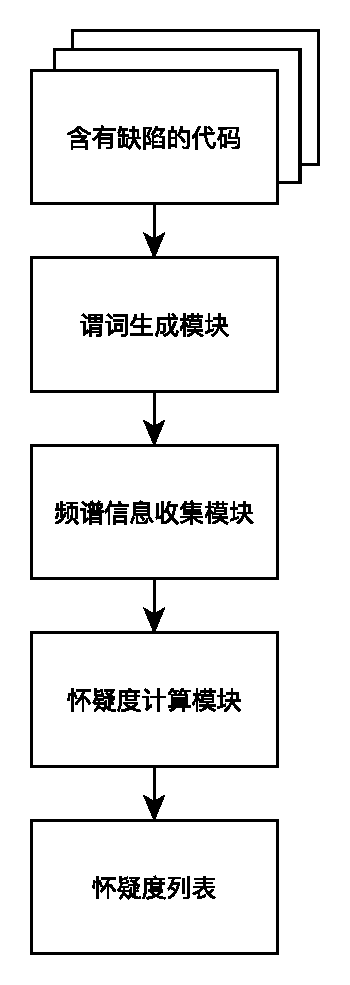
\includegraphics[width=5cm]{figure/frame1} 
\caption{缺陷定位框架模块图} 
\label{fl_frame1}
\end{figure}

谓词生成模块生成预定义的谓词,或者利用机器学习模型预测出谓词。
频谱信息收集模块把生成的谓词插装到缺陷代码,执行测试用例,收集测试用例覆盖谓词真假分支的情况。
最后怀疑度计算模块利用频谱信息,带入公式中计算怀疑度。

具体的流程图如图\ref{fl_frame2}所示。下面将会具体讲述这些步骤的实现。

\begin{figure}[htbp] 
\centering 
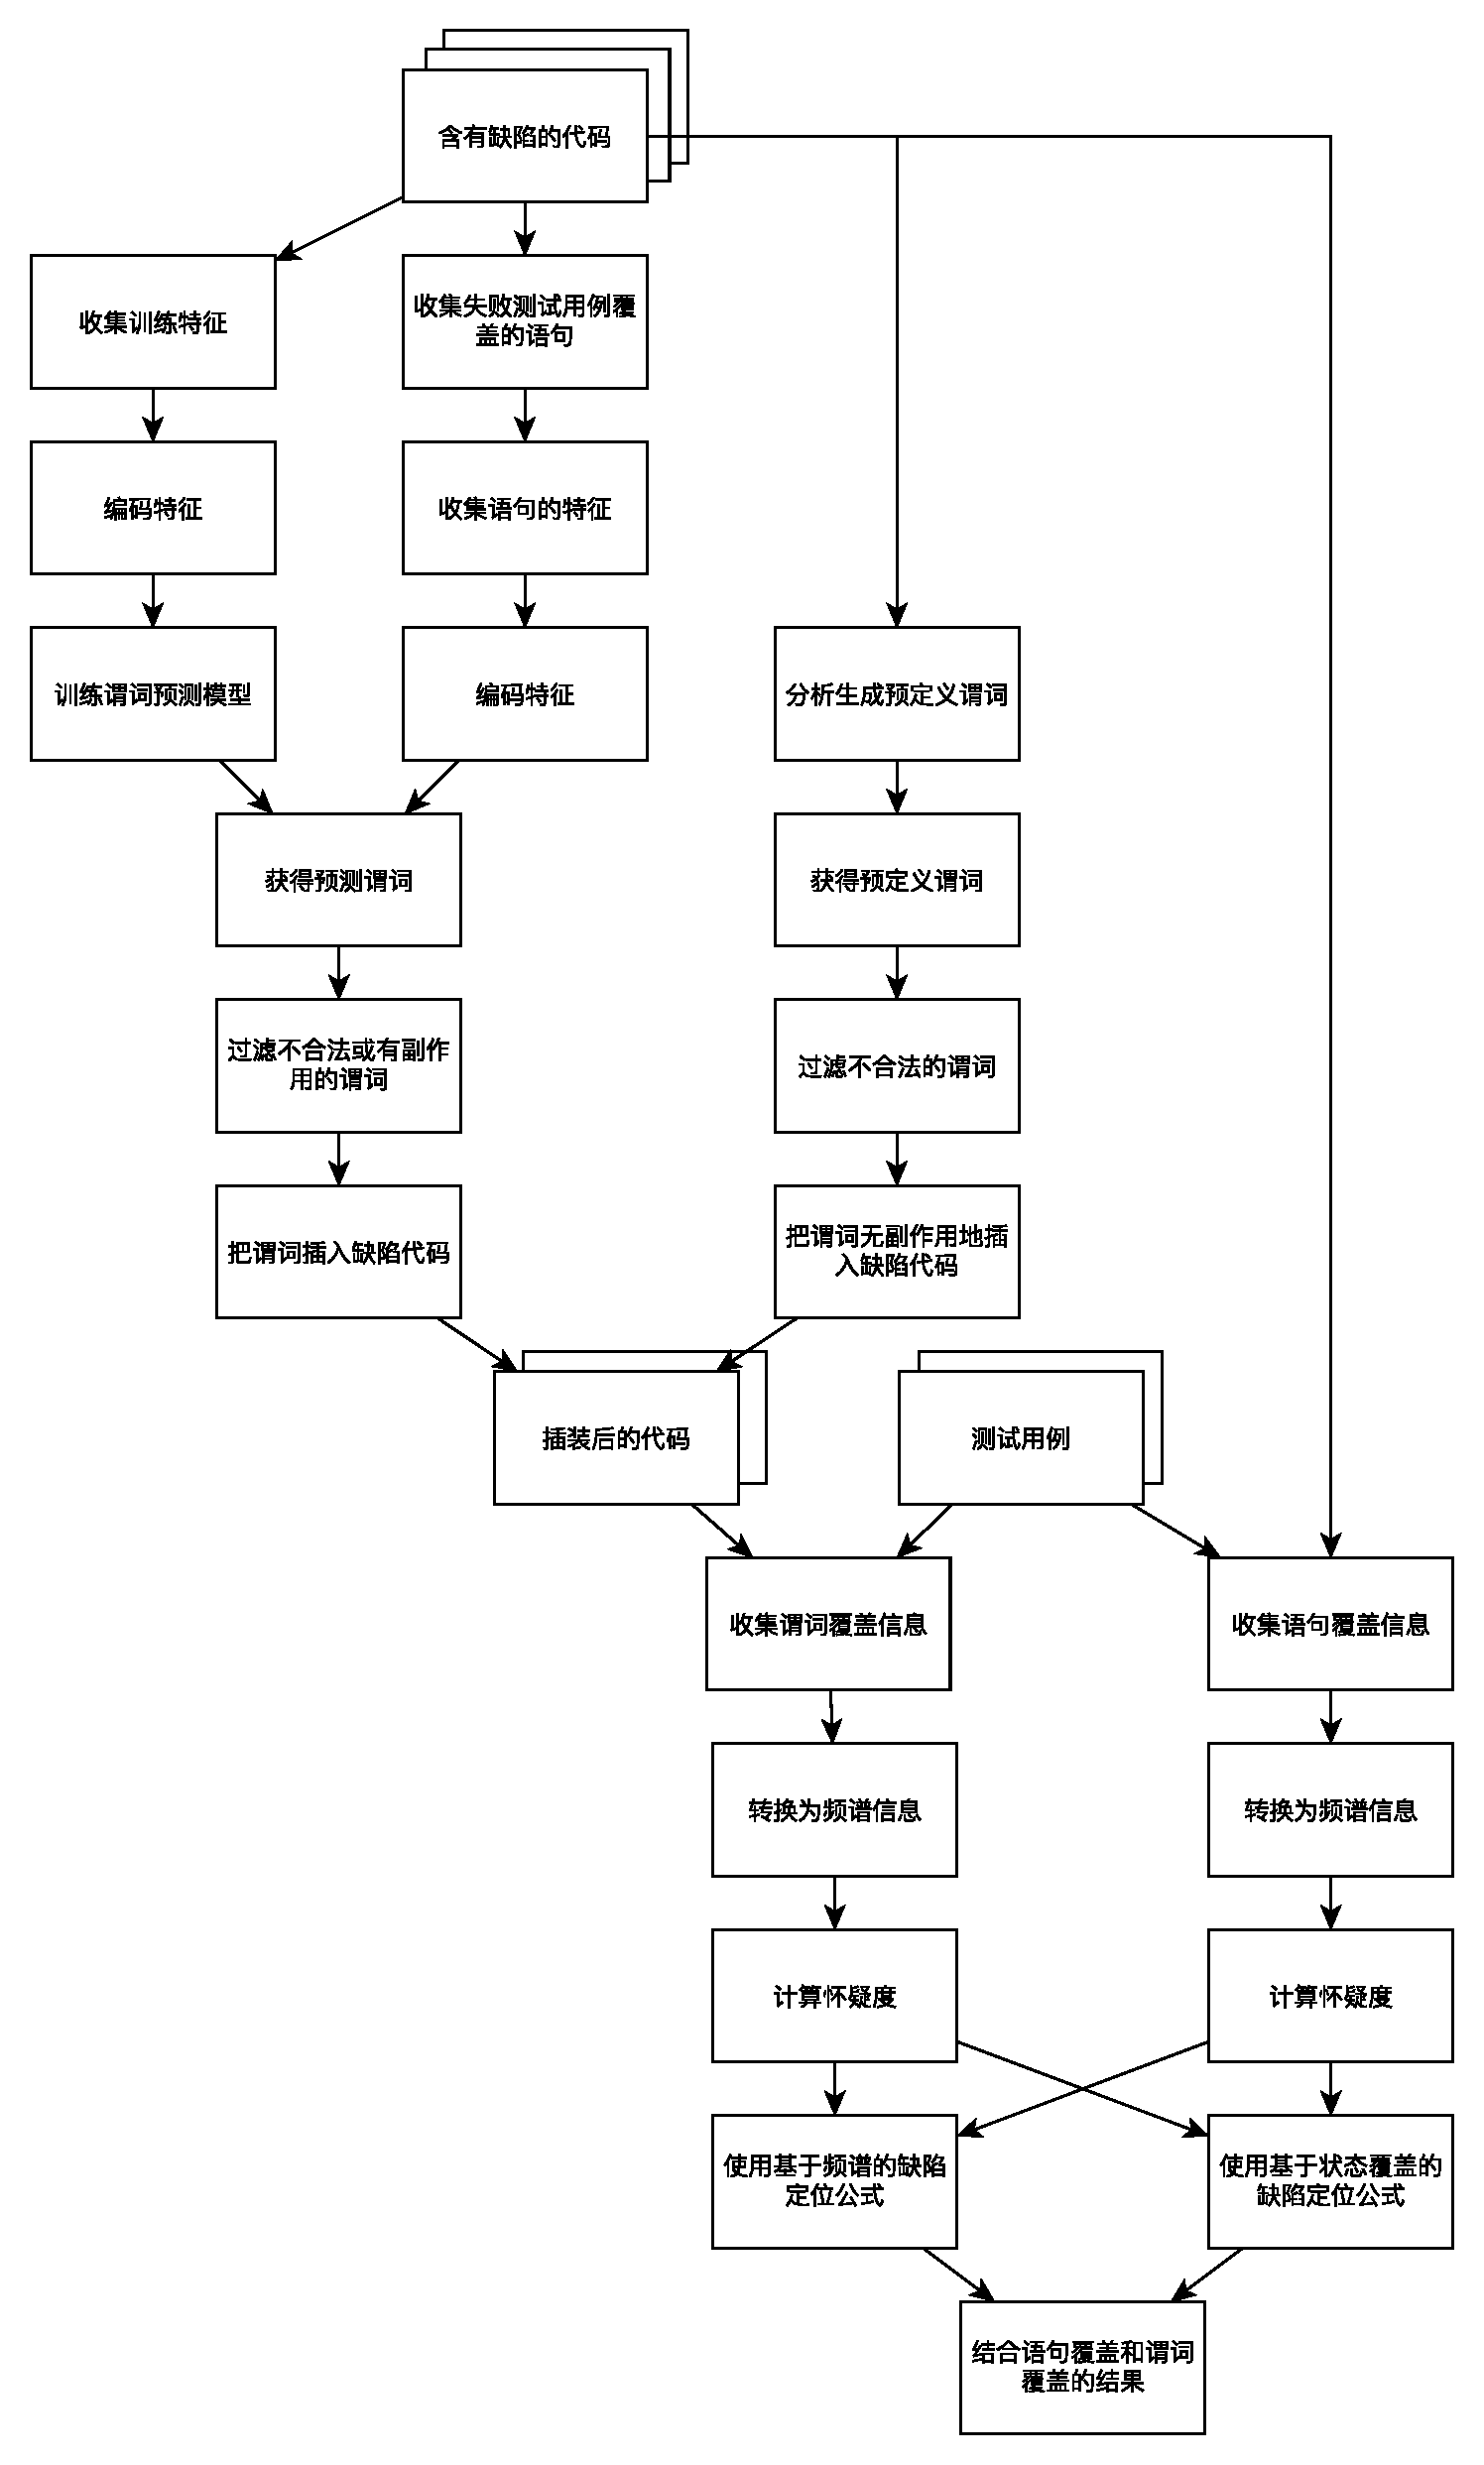
\includegraphics[width=13cm]{figure/frame2} 
\caption{缺陷定位整体流程图}
\label{fl_frame2}
\end{figure}

\section{谓词生成模块}

谓词生成模块负责生成后续会使用的谓词.
谓词生成模块分为两种,一种是生成预测谓词,一种是生成预定义谓词。
生成谓词的语句都是被失败的测试用例覆盖的语句。

\subsection{生成预测谓词模块}
\label{sec:gen_pred_impl}

生成预测谓词使用的是机器学习模型,使用Java和Python实现。
首先,Java代码通过JDT遍历缺陷代码的抽象语法树,提取表\ref{var_feature}中的特征。
这些特征被写入到磁盘上的 csv 文件中。
Python程序则读入 csv 文件中的特征,对特征进行编码和训练。

编码阶段,先对变量名、文件名、函数名使用scikit-learn\footnote{\url{http://scikit-learn.org/}}的K-Means聚类,其值转为类编号。
聚类模型等被存储到磁盘。
使用 scikit-learn 的 \mycode{LabelEncoder} 对特征 FileName,MethodName,VarName,VarType,LastAssign,BodyUse
和 OutUse 进行编码,归一化为数字,然后使用 \mycode{OneHotEncoder} 转为独热编码。

训练阶段,特征被放入神经网络或者随机森林中。
神经网络使用的全连接神经网络,用TensorFlow\footnote{\url{https://www.tensorflow.org/}}的 \mycode{DNNClassifier} 实现。
TensorFlow 是一个采用数据流图用于数值计算的开源软件库。
图中的节点表示数学操作,图中的线则表示在节点间相互联系的多维数据数组。
网络的输入使用 TensorFlow 的 \mycode{numpy\_input\_fn}。
使用这个函数的好处是,输入不需要在一开始的时候就被存储在内存,
而是在需要的时候才生成一个批(batch)的数据。
每次训练以一个批的数据为一次迭代。
VAR模型和EXPR模型的批尺寸(batch size)都为128。
输入数据会被随机打乱(shuffle)。
一个周期(epoch)就是把全部数据输入神经网络训练一次。
输入数据按照$7:3$的比例分为训练集和验证集。
训练时,会先使用训练集训练\mycode{INIT\_EPOCHS}个周期。
这是因为训练开始时,损失变化较大。
此后每次都再输入一个周期,并收集训练集和验证集在输入这个周期后的新模型上的损失和准确率。
程序会收集最近的\mycode{1}到\mycode{2 * TEST\_EPOCHS}个周期的
训练集和验证集的损失,记为$L(i, j)$。
其中$i$表示是最近的第$i$个周期的损失,$j$为$true$的话表示是训练集的损失,为$false$表示是验证集的损失。
然后分别计算\mycode{1}到\mycode{TEST\_EPOCHS},\mycode{TEST\_EPOCHS + 1}到\mycode{2 * TEST\_EPOCHS}
的训练集总损失值
$$
Loss_1 = \mathrm{Loss}(1, TE, true)
$$
$$
Loss_2 = \mathrm{Loss}(TE + 1, 2 * TE, true)
$$
和验证集的总损失值
$$
Loss_3 = \mathrm{Loss}(1, TE, false)
$$
$$
Loss_4 = \mathrm{Loss}(TE + 1, 2 * TE, false)
$$。
其中$TE$表示\mycode{TEST\_EPOCHS},
$\mathrm{Loss}$定义如下:
$$
\mathrm{Loss}(start, end, j) = \sum_{i=start}^{end}{L(i, j)}
$$。
终止训练的条件为
$$
Loss_1 < Loss_2 \ \mathrm{and} \ Loss_3 > Loss_4
$$。
也就是说当训练集的损失仍在下降,但是验证集的损失却开始上升时,
说明出现了过拟合,停止训练。
实现上会使用四个大小为\mycode{TEST\_EPOCHS}的队列,两个存放训练集损失,两个存放验证集损失。
比如对训练集来说,
一个存放\mycode{1}到\mycode{TEST\_EPOCHS}的数据,称为队列1。
一个存放\mycode{TEST\_EPOCHS + 1}到\mycode{2 * TEST\_EPOCHS},称为队列2。
每新训练完一个周期,得到当前的损失$l_0$,
再从队列1中弹出一个数据$l_1$,从队列2中弹出一个数据$l_2$。
于是,把$l_0$加入队列1中,并更新$Loss_1$:
$$
Loss_1 = Loss_1 - l_1 + l_0
$$。
把$l_1$加入加入队列2中,并更新$Loss_2$:
$$
Loss_2 = Loss_2 - l_2 + l_1
$$。
训练时会记录当前最小的验证集损失,并会把对应的模型存入磁盘。
训练停止后,最小损失对应的模型成为最终模型。
训练使用 \mycode{DNNClassifier} 的 \mycode{train} 方法,
验证损失和准确率使用 \mycode{evaluate} 方法。
神经网络使用的优化算法是 \mycode{ProximalAdagradOptimizer},
初始学习率设置为0.05,L2正则惩罚系数为0.0001。
随机森林使用 scikit-learn 中的随机森林 \mycode{RandomForestClassfier} 。
训练使用其 \mycode{fit} 方法。
训练好的模型被保存在磁盘中。
神经网络模型直接通过设置 \mycode{model\_dir} 参数保存,
随机森林模型使用 pickle\footnote{\url{https://docs.python.org/3/library/pickle.html}} 保存。

预测阶段,对收集的失败测试用例覆盖的语句进行谓词预测。
首先用Java的JDT提取语句中左值变量的特征,然后写入磁盘上的 csv 文件。
Python程序读入 csv 文件中的特征和编码阶段存储的聚类模型。
同时Python程序也会读入训练时使用的 csv 文件,以获取同样的 \mycode{LabelEncoder} 和 \mycode{OneHotEncoder}。
使用聚类模型对特征的变量名、函数名和文件名划入某个已有的分类。
然后用和训练时一样的 \mycode{LabelEncoder} 和 \mycode{OneHotEncoder} 对特征 FileName,MethodName,VarName,VarType,LastAssign,BodyUse
和 OutUse 进行编码。
最后把预测变量的特征传入训练好的VAR模型和EXPR模型中预测。
神经网络通过 \mycode{predict} 方法预测。
该方法返回预测结果的一个列表。
列表中一个元素对应于一个预测输入,该元素的 \mycode{probabilities} 域表示这个样本属于各个标签的概率,
\mycode{classes} 域表示表示这个样本的预测标签。
随机森林通过 \mycode{predict\_proba} 方法预测,得到一个矩阵。每行对应一个样本,每列对应这个样本属于某个标签的概率。
VAR模型会输出这个变量出现在谓词中的概率,EXPR模型会对一个样本的概率值排序,取概率最高的200个输出。
最后,将同一个变量其VAR模型的输出$P_{var}$和EXPR模型的输出$P_{pred_i}$相乘,把联合概率大于$0.005$的变量及谓词输出。

验证阶段是在正常的缺陷定位中不存在的阶段。
在测试中被用于测试模型的预测准确性。
在验证阶段,输入数据会被使用 scikit-learn 的 \mycode{train\_test\_split} 函数随机分为60\%的训练集,20\%的验证集和20\%的测试集。
然后使用训练集和验证集去训练模型,对得到的模型使用测试集验证其准确率。
神经网络的准确率计算使用 \mycode{DNNClassifier} 自带的 \mycode{evaluate} 方法
的域 \mycode{accuracy} 获得。
随机森林的准确率使用 \mycode{RandomForestClassfier} 自带的 \mycode{score} 方法获得。
而两者的其他评估数值由 scikit-learn 提供的计算接口获得。

过滤阶段,过滤掉预测出不合法或有副作用的谓词。
使用JDT遍历谓词过滤。
静态分析过滤后的谓词还会被单个编译过滤。
每条语句最终只有过滤后的五个概率最高的谓词和它们的相反谓词。

\subsection{生成预定义谓词模块}

生成预定义谓词使用Java的JDT遍历抽象语法树。

对于一个返回语句,只要其返回值不是空 \mycode{return;},就生成谓词。
对于条件语句 \mycode{if, for, while, do, switch},生成其条件表达式的谓词。
对于赋值语句和变量声明语句,如果其左值是基本数据类型,获取当前行可见的其他同类型变量,生成谓词。

预定义生成的谓词数量往往大于预测谓词的数量。
过滤的时候使用编译过滤速度较慢。
其实预定义谓词并不需要过滤。
首先,条件语句的谓词就是其条件表达式和其条件表达式取反,这种谓词肯定是编译正确的,所以不需要过滤。
对于返回语句来说,只要验证 \mycode{v > 0} 是否编译正确就可以知道 \mycode{v < 0} 等谓词是否编译正确。
对于数值对来说,只要验证 \mycode{a > b} 是否编译正确就可以知道 \mycode{a < b} 等谓词是否编译正确。
因此减少过滤的谓词数量。

\section{频谱信息收集模块} 

频谱信息收集模块主要分为两步,第一步是把谓词插入到代码中,第二步是执行测试用例收集执行信息。

插入谓词分为两种情况,一种是插入预测的谓词,一种是插入预定义的谓词。
插入预测的谓词采用普通的插入方法,而插入预定义的谓词采用无副作用的插入方法。
这两种方法都是使用JDT遍历抽象语法树,然后对函数声明 \mycode{MethodDeclaration} 节点进行一个对其字节点的递归遍历。
这是因为插入谓词涉及到修改语法树,因此对于一个要被修改的节点来说,其父节点是被需要的甚至也是要修改的。

插入预测谓词时直接插入即可。而插入预定义谓词时,可能会涉及到新建变量、修改原有语句等。
因为无副作用的插入方法会新建一个中间变量,然后用这个中间变量替换原有变量的位置。
比如,为了在 \mycode{return a.increase();} 处插入谓词 \mycode{a.increase() > 0},
首先是使用 \mycode{VariableDeclarationFragment} 新建一个变量,这个变量的变量名组成为
\mycode{"automatic\_" + lineNumber + "\_" + varCount}。
其中 \mycode{lineNumber} 是行号, \mycode{varCount} 是一个递增的新变量计数。
然后把这个 \mycode{VariableDeclarationFragment} 放入更高一层的 \mycode{VarableDeclarationExpression} ,
得到 \mycode{int automatic\_11\_2}。
再将其放入 \mycode{Assignment},得到 \mycode{int automatic\_11\_2 = a.increase();}。
把原本的返回语句改为 \mycode{return automatic\_11\_2;}。
然后谓词也要修改,
原本要插入的谓词是 \mycode{a.increase() > 0},
现在要插入的谓词应该是 \mycode{automatic\_11\_2 > 0}。

为了收集执行信息,需要在代码中加入一些计数、标记、打印的语句。
为了方便起见,这些方法被包装在一个负责收集这些信息的类的静态方法中,
而这个类会被放入到缺陷代码的源代码中。

在代码被插入谓词和记录频谱的语句后,使用测试用例执行代码。
频谱信息会被输出到文件中。
频谱信息分为两类,第一类是SOBER算法的频谱信息。
SOBER算法的每个谓词会对应若干个覆盖信息。
每一条覆盖信息对应一个测试用例的覆盖情况,包含三个数值,分别是谓词为真的次数、谓词为假的次数和当前测试用例是通过还是失败。
第二类是除SOBER以外的公式的频谱信息。
每个谓词对应一条覆盖信息,包含四个数值,分别是谓词真分支被覆盖的失败测试用例个数、谓词真分支被覆盖的通过测试用例个数、谓词(无论真假分支)被覆盖的失败测试用例个数和谓词(无论真假分支)被覆盖的通过测试用例个数。

除了收集谓词的覆盖情况外,还会收集语句的频谱信息,
包括语句被覆盖的失败测试用例个数和被覆盖的通过测试用例个数。

\section{怀疑度计算模块}

怀疑度计算模块根据频谱信息的不同也分为两种。
一种是SOBER算法的怀疑度计算,一种是其他算法的怀疑度计算。
在实现上,SOBER算法继承一个父类,其他算法继承另一个父类。
子类需要实现两个函数,一个是 \mycode{getName} 返回算法名,
一个是 \mycode{getScore} 返回怀疑度。
父类负责从磁盘读取执行信息并处理为频谱信息,计算并结合语句的怀疑度和谓词怀疑度,根据怀疑度对语句进行排序,最后输出到磁盘。
% 具体的结合方式根据会在

在一条语句的多个谓词中,选择怀疑度最高的作为这个语句的最终谓词怀疑度。结合方式有\textsc{MaxPred}和\textsc{LinPred}。



	\chapter{实验与验证}

\section{研究问题}

本文提出了一个结合了基于频谱的缺陷定位和基于状态覆盖的缺陷定位的缺陷定位框架,
并且通过结合深入分析基于频谱的缺陷定位和基于状态覆盖的缺陷定位能够准确定位的原因。

本文试图回答以下几个问题:
\begin{enumerate}
\item \textbf{当使用不同的数据收集粒度时,缺陷定位技术的效果有什么不同?} \\
这个研究问题探索了数据收集的粒度对缺陷定位结果的影响。
最近研究使用的方法级别的缺陷定位从两个维度收集数据:
语句级别和方法级别。
但是没有现有方法探究了数据收集粒度对缺陷定位结果的影响。
因为从不同的粒度收集数据会导致谓词数量的不同,
而谓词数量对执行时间影响程度也不清楚。
\item \textbf{不同的怀疑度计算公式会如何影响缺陷定位的结果?} \\
这个研究问题探索了缺陷定位公式的重要性,
并分析了是否还能通过改进缺陷定位公式去提升缺陷定位效果,
为后续研究提供了参考。
\item \textbf{缺陷定位技术的不同结合方式效果如何?} \\
在章\ref{sec:approach_comb}中,
本文探讨了结合缺陷定位技术的方法。
这个研究问题研究了不同结合方式的效果。
\item \textbf{机器学习模型预测谓词的准确率如何?} \\
这个研究问题探索了谓词预测模型的准确率,
并且在不同的机器学习模型上进行了对比。
\item \textbf{哪种谓词能够更好地帮助定位?} \\
这个研究问题比较了基于谓词预测的缺陷定位和本文提出的结合方法、现有方法之间的结果,
分析谓词在定位缺陷中的作用和不足。
% \item \textbf{和现有很多缺陷定位方法相比,本文的方法效果如何?} \\

\end{enumerate}

\section{实验数据}

本文使用Defects4j数据集\parencite{Just2014Defects4J}(v1.0)作为实验对象,
下文所提到的Defects4j都是 v1.0 版本。
Defects4j数据集含有357个真实的缺陷,来自五个大型的开源软件项目,见表\ref{defects4j_details}。
其中,“实验缺陷数目”是本文在实验中实际使用了的缺陷数目,“代码行数(千行)”表示的是这五个项目最近的版本的代码行数。
本文只使用了330个缺陷是因为其余27个缺陷因为插装后的代码太大导致“code too large"的报错而无法运行。

\begin{table}
\centering
\begin{tabular}{|l|r|r|r|r|}
\hline
项目名称 & 缺陷数目 & 实验缺陷数目 & 代码行数(千行) & 测试用例数目 \\
\hline
JFree\textbf{Chart} & 26 & 26 & 96 & 2205 \\
\hline
\textbf{Closure} compiler & 133 & 122 & 90 & 7927 \\
\hline
Apache commons-\textbf{Math} & 106 & 98 & 85 & 3602 \\
\hline
Apache commons-\textbf{Lang} & 65 & 57 & 22 & 2245 \\
\hline
Joda-\textbf{Time} & 27 & 27 & 28 & 4130 \\
\hline
总计 & 357 & 330 & 321 & 20109 \\
\hline
\end{tabular}
\caption{Defects4j数据集缺陷情况}
\label{defects4j_details}
\end{table}

\section{实验标准}

为了验证本文提出的结合后的缺陷定位的效果,以及预测谓词的效果,
需要一套衡量缺陷定位效果的标准和预测谓词效果的标准。

\subsection{缺陷定位结果标准}

本文使用两种常用的缺陷定位标准: Top-k 的召回率和 EXAM 分数。

Top-k 的召回率衡量的是有多少缺陷能够排在怀疑列表的前k位。
根据Kochhar等人的研究\parencite{Kochhar2016Practitioners},
超过73\%的参与者认为观察怀疑列表的前5个程序元素是可以接受的,
几乎所有参与者都认为10个程序元素是可以接受的最大的需要观察的程序元素个数。
所以本文采用1,3,5,10作为k值。
对于怀疑度分数相同的程序元素,它们的排名会使用平均排名,这也是很多已有研究使用的方法\parencite{Pearson2017Evaluating,Xuan2014Learning,Steimann2013Threats,Wong2016A}。

EXAM 分数衡量的是开发者需要查看多少个位置才能看到真正的缺陷。
$$
\mathrm{EXAM} = \frac{n}{N}
$$
其中$N$表示候选的程序元素个数(比如被失败的测试用例覆盖的语句),$n$表示缺陷程序元素排在怀疑度列表的第$n$位。
EXAM 分数是一个0到1之间的值,且值越小越好。
它反映出了含有缺陷的程序元素在所有可疑程序元素中的相对位置,
体现出整个缺陷定位方法的效果。
很多工作都使用了这个方法\parencite{Wong2012Effective,Pearson2017Evaluating}。

\subsection{谓词预测结果标准}

本文对谓词预测结果的评判方法采用机器学习分类问题的评判方法。

首先引入一些评估分类问题效果时需要的统计量。
混淆矩阵统计量见表\ref{confusion_matrix}。
样本总数为$N$。
正例反例为两个相对的概念。
对于多分类问题,其余分类都为反例。

\begin{table}
\centering
\begin{tabular}{|c|c|c|}
\hline
\multirow{2}*{真实情况} & \multicolumn{2}{|c|}{预测结果} \\
\cline{2-3}
~ & 正例 & 反例 \\
\hline
正例 & TP(真正例) & FN(假反例) \\
\hline
反例 & FP(假正例) & TN(真反例) \\
\hline
\end{tabular}
\caption{分类结果混淆矩阵}
\label{confusion_matrix}
\end{table}

准确率(accuracy)衡量的是分类正确的样本数占样本总数的比例:
$$
\mathrm{Accuracy} = \frac{TP + TN}{N} = \frac{TP + TN}{TP + FN + FP + TN}
$$
。

准确率能够衡量一个机器学习模型的预测情况,但是有的时候只有准确率还不够。
有的时候人们还关心查准率和召回率。

查准率(precision)衡量的是被分类为正例的样本中有多少是真的正例:
$$
\mathrm{Precision} = \frac{TP}{TP + FP}
$$。

查全率或召回率(recall)衡量的是正例中有多少被分类为正例:
$$
\mathrm{Recall} = \frac{TP}{TP + FN}
$$。

查准率和查全率是一对相互矛盾的度量。
一般来说,查准率高时,查全率低,而查准率低时,查全率高。
F1 度量结合查准率和查全率,给出一个便于比较的统一的值:
$$
\mathrm{F1} = \frac{2 \times \mathrm{Precision} \times \mathrm{Recall}}{\mathrm{Precision} + \mathrm{Recall}}
$$。

对于二分类问题来说,正例负例就是二分类的两个类别。
但是对于多分类来说,每个类都可以是正例,这时其余类别就是负例。
所以多分类问题的查准率,查全率和 F1 的对数和分类的类别数量一致。
如果分类的类别数量非常多,观察庞大的查准率、查全率和 F1 并不能直观地描述预测结果,
需要将各个分类的查准率、查全率和 F1 结合起来。
$TP_i,FN_i,FP_i,TN_i$表示多分类问题下,分类$i$的真正例、假反例、假正例和真反例的数目。
分类数记为$C$,$c_i$表示分类为$i$的样本数量。
多分类问题的查准率、查全率和 F1 有以下几种结合方式:
\begin{itemize}
\item \textbf{micro}:\\
先在全局的角度计算真正例、假反例和假正例的个数,然后带入公式计算查准率、查全率和 F1。
以查准率为例:
$$
\mathrm{Precision} = \frac{\sum_{i=1}^C{TP_i}}{\sum_{i=1}^C{(TP_i + FP_i)}}
$$。
\item \textbf{macro}:\\
先收集每个分类的真正例、假反例和假正例的个数,带入公式计算每个分类的查准率、查全率和 F1,最后求均值。
这个不会考虑标签的不均衡。
以查准率为例:
$$
\mathrm{Precision_i} = \frac{TP_i}{TP_i + FP_i}
$$
$$
\mathrm{Precision} = \frac{1}{C}\sum_{i=1}^c{\mathrm{Precision_i}}
$$。
\item \textbf{weighted}:\\
先收集每个分类的真正例、假反例和假正例的个数,带入公式计算每个分类的查准率、查全率和 F1,最后根据
分类的支持度(该分类的样本在总样本中所占的数目)分配权重求均值。
这个算法与 macro 相比,考虑了标签的不均衡性。
以查准率为例:
$$
\mathrm{Precision_i} = \frac{TP_i}{TP_i + FP_i}
$$
$$
\mathrm{Precision} = \sum_{i=1}^c{\frac{c_i}{C}\mathrm{Precision_i}}
$$。
\end{itemize}

本文采用weighted的方式得到多分类问题的查准率、查全率和F1。

\section{实验设置}

\subsection{数据收集粒度}

本文考虑两种数据收集粒度:语句级别和函数级别。
因为本文关注于函数的缺陷定位,所以对于函数级别的数据收集,
只需要直接在函数的出入口收集就可以。
而对于语句级别的数据收集,则需要取一个函数内所有语句的最大怀疑度值作为这个函数的怀疑度。
本文默认配置使用语句级别的数据收集。

\subsection{怀疑度公式}
\label{sec:exp_all_formula}

怀疑度的公式上,本文实现了七种怀疑度计算的公式。
五种是经典的基于频谱的缺陷定位公式见表\ref{susp_formula},
两种是基于频谱的缺陷定位的公式\ref{eq:sd}和公式\ref{eq:sober}。
本文默认配置使用Ochiai作为怀疑度公式。

\subsection{结合怀疑度的方法}

在章\ref{sec:approach_comb}的讨论中,
本文使用了公式
$$
c(s,e,r) = max_{p \in s(e)}r(p)
$$
计算得到了程序元素$e$的怀疑度,
并提出了\textsc{MaxPred}和\textsc{LinPred}两种结合方式。

在本文的实验中,默认配置使用$\alpha = 0.5$的\textsc{LinPred}。
其中,第一个怀疑度使用基于频谱的缺陷定位计算得到($s_0(e)$产生的谓词恒为\mycode{true}),
第二个使用基于状态覆盖的缺陷定位的谓词计算得到。

\subsection{谓词}

为了探索谓词在缺陷定位中的作用,本文把谓词分为三大类:预定义谓词、预测谓词和恒真谓词。
对预定义谓词,又根据其定义分为三类:分支、返回和数值对。
在本文的试验中,默认配置使用预定义谓词。

\section{实验结果与分析}

\subsection{不同数据收集粒度对比}

本小节试图通过探索不同数据收集粒度对缺陷定位效果效率的影响,来回答第一个研究问题。
对于两种不同的数据收集粒度,我们都进行了实验。
在语句级别收集数据的方法和此前的统计性调试的方法一样。
而在函数级别收集数据的时候,谓词的类型会有差别。
首先是没有“分支”类型的谓词。
然后在收集“数值对”这样的预定义谓词时,不存在对应的赋值语句,
所以转而收集所有可以访问的类成员变量和函数参数的“数值对”。
“数值对”类型的谓词会被插入在函数入口和出口处。
“返回”类型的谓词会被插入在函数的出口处,如果函数有返回值的话。

实验结果如图\ref{fig:ms-level-compare}所示。
图中\textsc{LinPred}表示在语句级别收集数据,
\textsc{LinPred-m}表示在函数级别收集数据。
根据实验结果,我们可以发现\textsc{LinPred}的效果在
Top-k(k=1,3,5, 10)和 EXAM 分数上都优于\textsc{LinPred-m}的效果。
具体来说,在Top-1指标上,\textsc{LinPred}相比于\textsc{LinPred-m}提升了$67.1\%$。

\finding{更细粒度的数据收集会让缺陷定位效果变好。}

\begin{figure}[htbp] 
\centering 
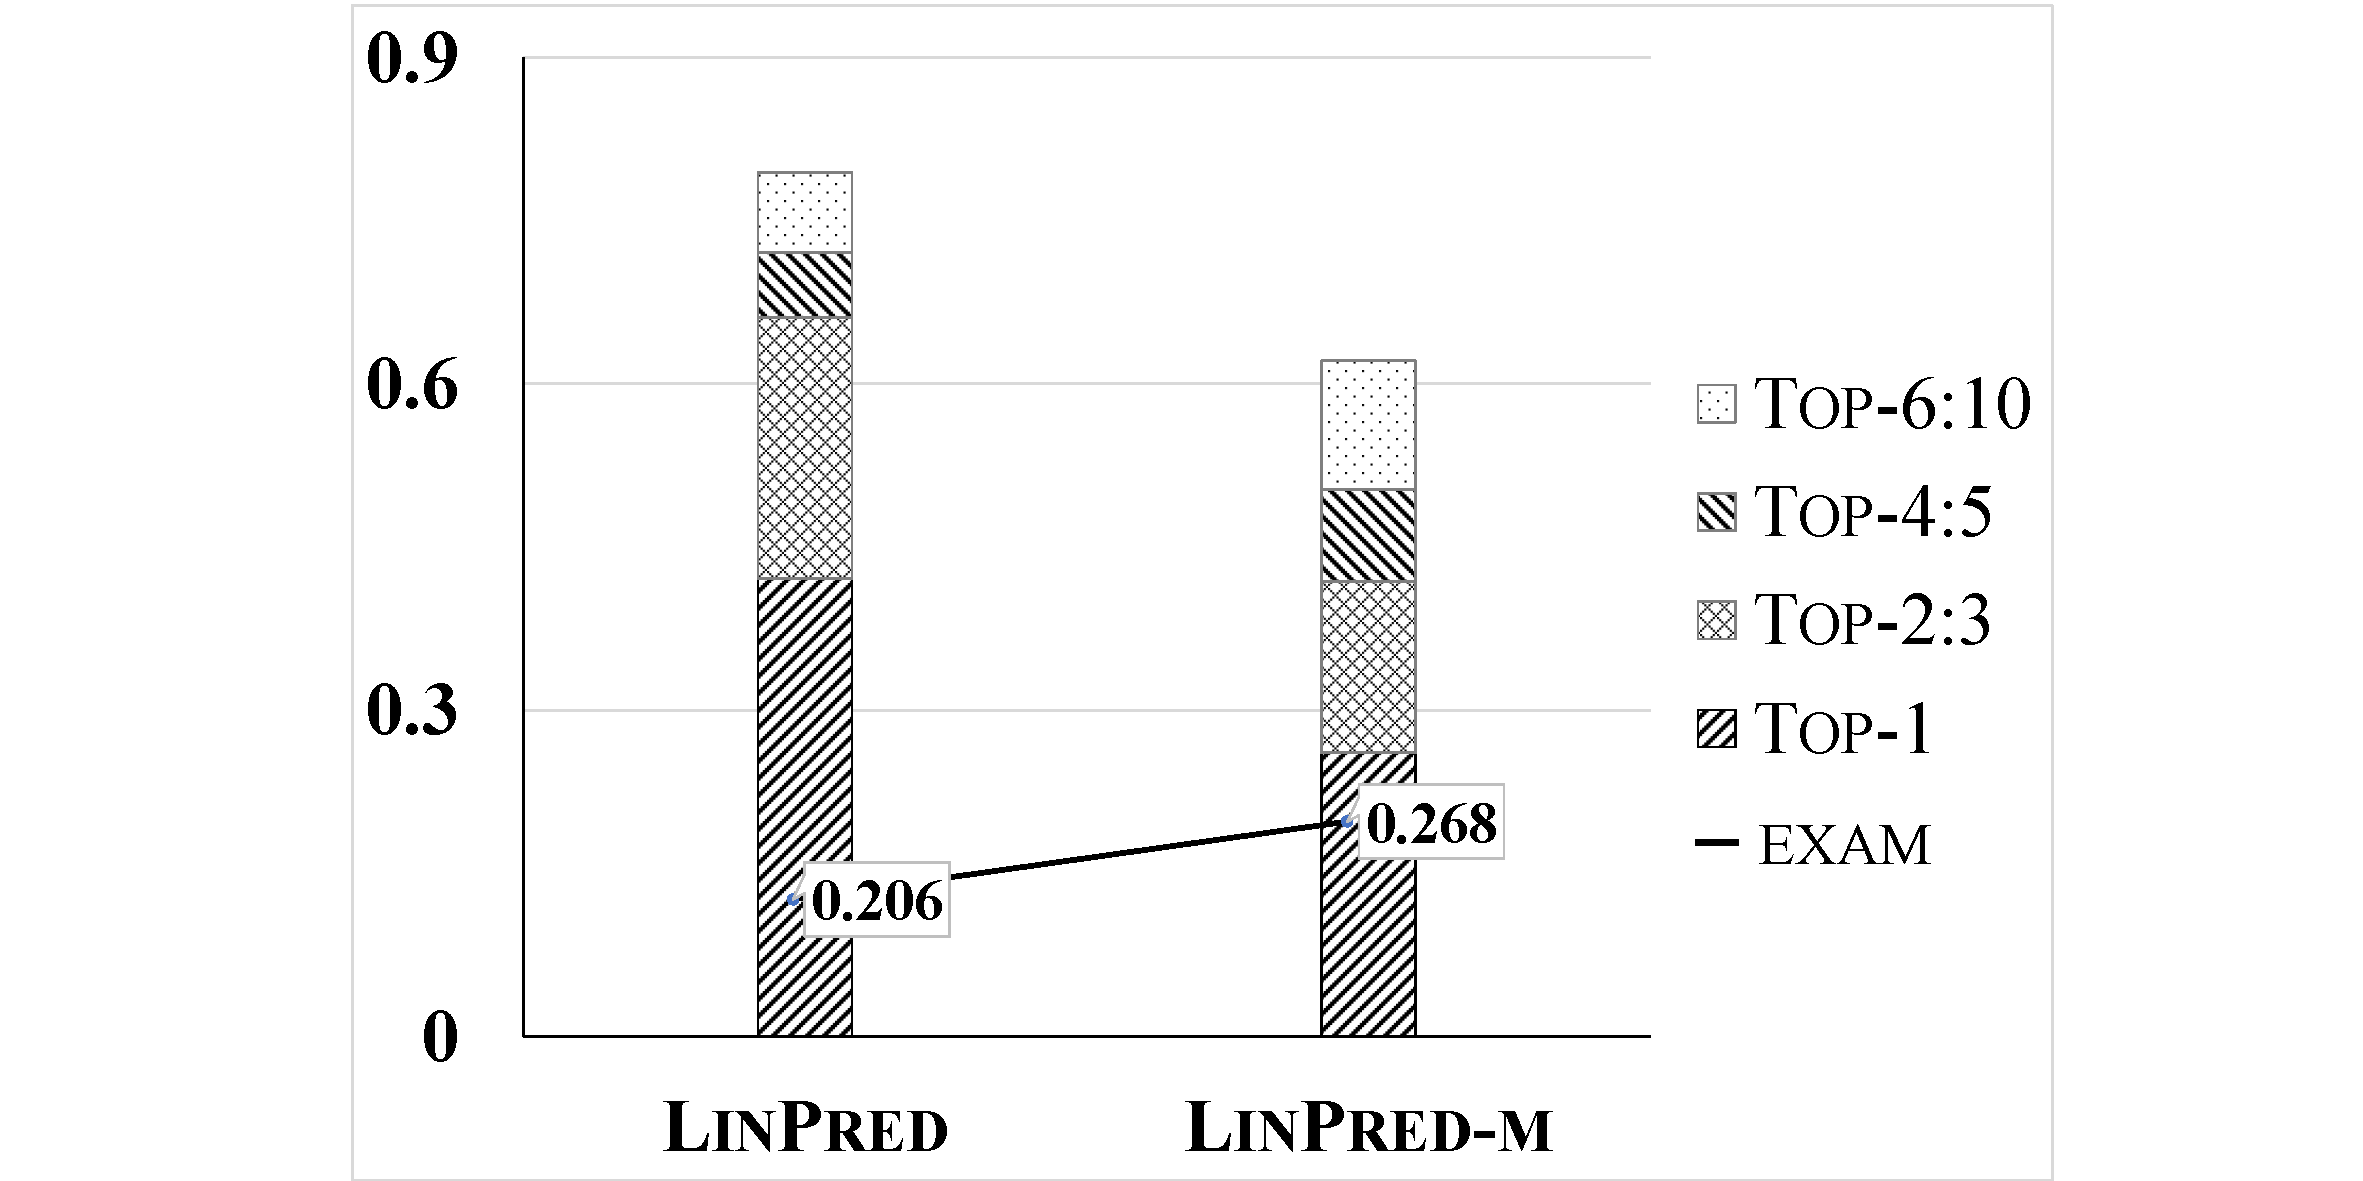
\includegraphics[width=12cm]{figure/ms-level-compare} 
\caption{语句级别和函数级别数据收集的缺陷定位效果对比} 
\label{fig:ms-level-compare}
\end{figure}

数据收集粒度变细之后,谓词数量会增多。
为了进一步探索增加谓词之后缺陷定位的效率是否会受到影响,
本文比较了在语句级别收集数据和在函数级别收集数据的执行时间。
我们发现,平均来说\textsc{LinPred}的谓词数量大约是\textsc{LinPred-m}谓词数量的4.1倍,
但是\textsc{LinPred}的执行时间只是\textsc{LinPred-m}的1.4倍。
同时,\textsc{LinPred}的执行时间也是平均在三分钟以内。
相比于提升数据收集粒度、降低谓词数量,在语句级别收集数据并不会严重地影响性能,同时能带来极大的效果提升。

\subsection{不同的怀疑度计算公式}

本小节将分析比较不同的怀疑度公式对缺陷定位结果的影响,并回答第二个研究问题。
在章\ref{sec:exp_all_formula}中,我们使用了七个怀疑度公式。
然而 SOBER 公式因为插装的内容较多,导致出现“code too large”的编译错误的项目较多,所以将 SOBER 公式排除。
因此剩下五种基于频谱的缺陷定位公式和一种基于状态覆盖的缺陷定位公式。

实验结果如图\ref{fig:formulas}。
图中展示的是每个怀疑度公式的 Top-k 和 EXAM 分数。
图中的“SD”表示的是统计性调试的结果。
从实验结果可以看出,前五个基于频谱的缺陷定位公式并没有太大的差别,
这和之前的研究结果一致。
统计性调试的结果则表现不理想。
可以发现基于频谱的缺陷定位公式的效果优于基于状态覆盖的缺陷定位公式效果。

\finding{基于频谱的缺陷定位公式的效果优于基于状态覆盖的缺陷定位公式效果}

\begin{figure}[htbp] 
\centering 
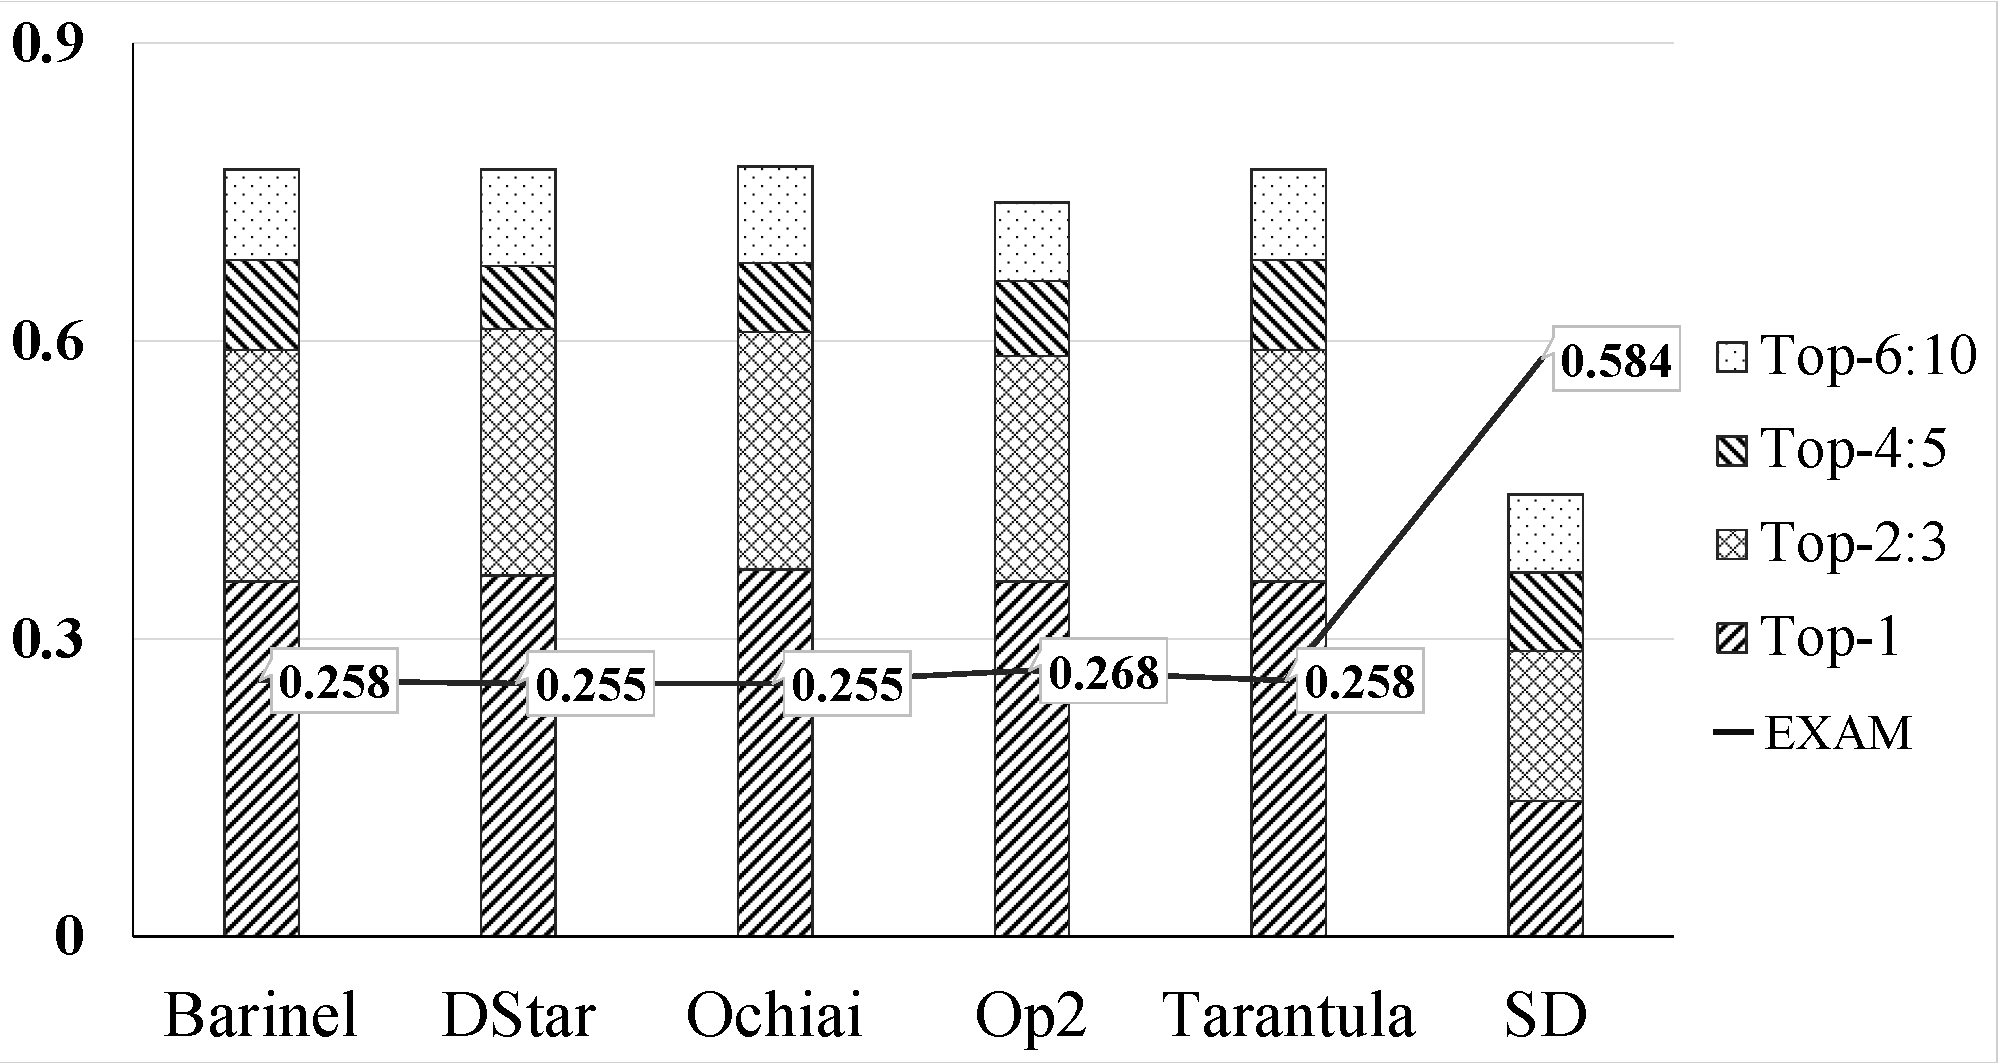
\includegraphics[width=12cm]{figure/formulas} 
\caption{不同怀疑度公式的效果对比} 
\label{fig:formulas}
\end{figure}

为了深入分析基于状态覆盖的缺陷定位公式效果不好的原因,
我们手动分析了统计性调试效果不好的缺陷。
我们发现这是由于很多缺陷都只有一个失败的测试用例,这导致一个谓词的真分支往往只被一个失败的测试用例覆盖。
这会导致统计性调试的公式中$t_f = 1$,导致$log(t_f) = 0$,然后$\frac{log(F)}{log(t_f)} = INF$,
于是最终计算得到的怀疑度为0。
这样谓词本身已经失去了甄别缺陷的能力,仅仅因为测试用例的数量就导致很多谓词的怀疑度为零。
而统计性调试在此前的实验中有效是因为此前的实验对象中一个缺项往往对应多个失败的测试用例。
比如在Liblit\parencite{Liblit2005Scalable}的实验中,对每一个研究对象生成32000个随机输入。
其测试用例数量远远大于 Defects4j 这样的实际项目。
而基于频谱的缺陷定位公式却仍然能够在失败测试用例数量少的情况下得到比较靠谱的结果,
因为它对失败测试用例数量的依赖没有基于状态覆盖的缺陷定位公式的高。
统计性调试公式仍然有它的应用场景。
在使用缺陷定位公式时,可以根据其应用场景选择合适的公式。

\subsection{不同的结合方式}

本小节将深入探讨不同的结合方式,来回答第三个研究问题。
结合的方式被分为了两种\textsc{MaxPred}和\textsc{LinPred}。
图\ref{fig:diff-comb-compare}展示了不同结合方式的 Top-k 和 EXAM 结果。
“SBFL”表示传统的基于频谱的缺陷定位的结果(谓词恒为真),这里的\textsc{MaxPred}的谓词使用预定义谓词。

\begin{figure}[htbp] 
\centering 
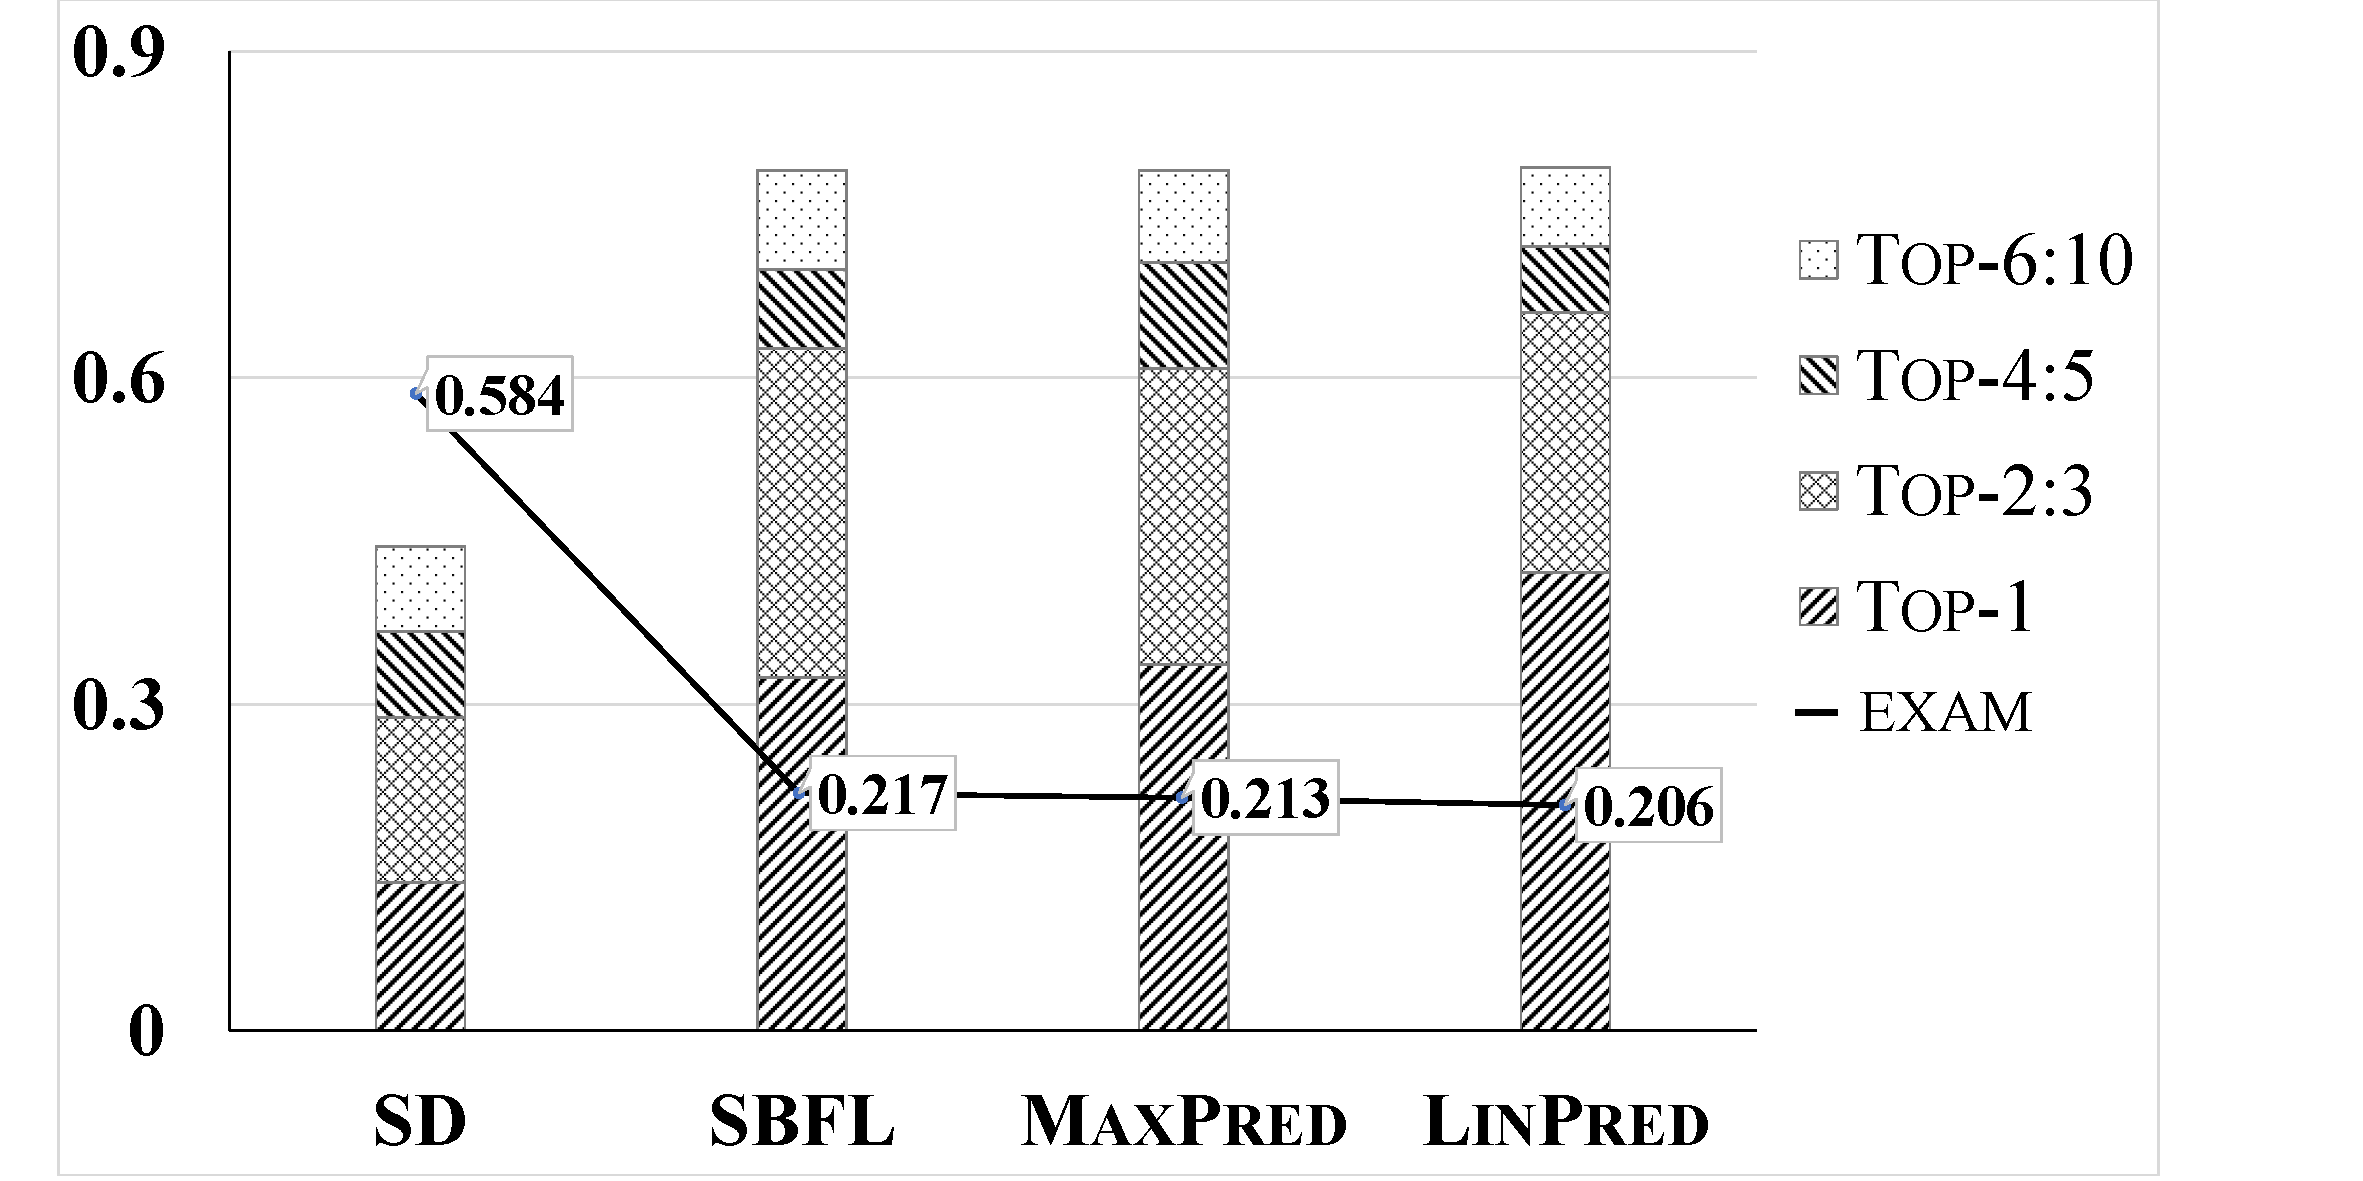
\includegraphics[width=12cm]{figure/diff-comb-compare} 
\caption{不同的结合方式的对比} 
\label{fig:diff-comb-compare}
\end{figure}

从图中可以看出,结合后的\textsc{MaxPred}和\textsc{LinPred}在 Top-1 上优于
原始的方法。
\textsc{LinPred}不仅获得了最好的 Top-k(k=1,3,5,10)值,还拥有最好的 EXAM 值。
\textsc{LinPred}在 Top-1 上与传统的统计性调试比提升了208.9\%,
与基于频谱的缺陷定位比提升了29.9\%。
可见 SBFL 和 \textsc{MaxPred} 结合之后的\textsc{LinPred}效果非常好。

图\ref{fig:diff-comb-compare}中的\textsc{LinPred}采用的默认的$\alpha = 0.5$。
为了分析 SBFL 和 \textsc{MaxPred} 哪一种对结果的影响更大,
采用不同的$\alpha$值进行实现,结果如图\ref{fig:coefficient}。

\begin{figure}[htbp] 
\centering 
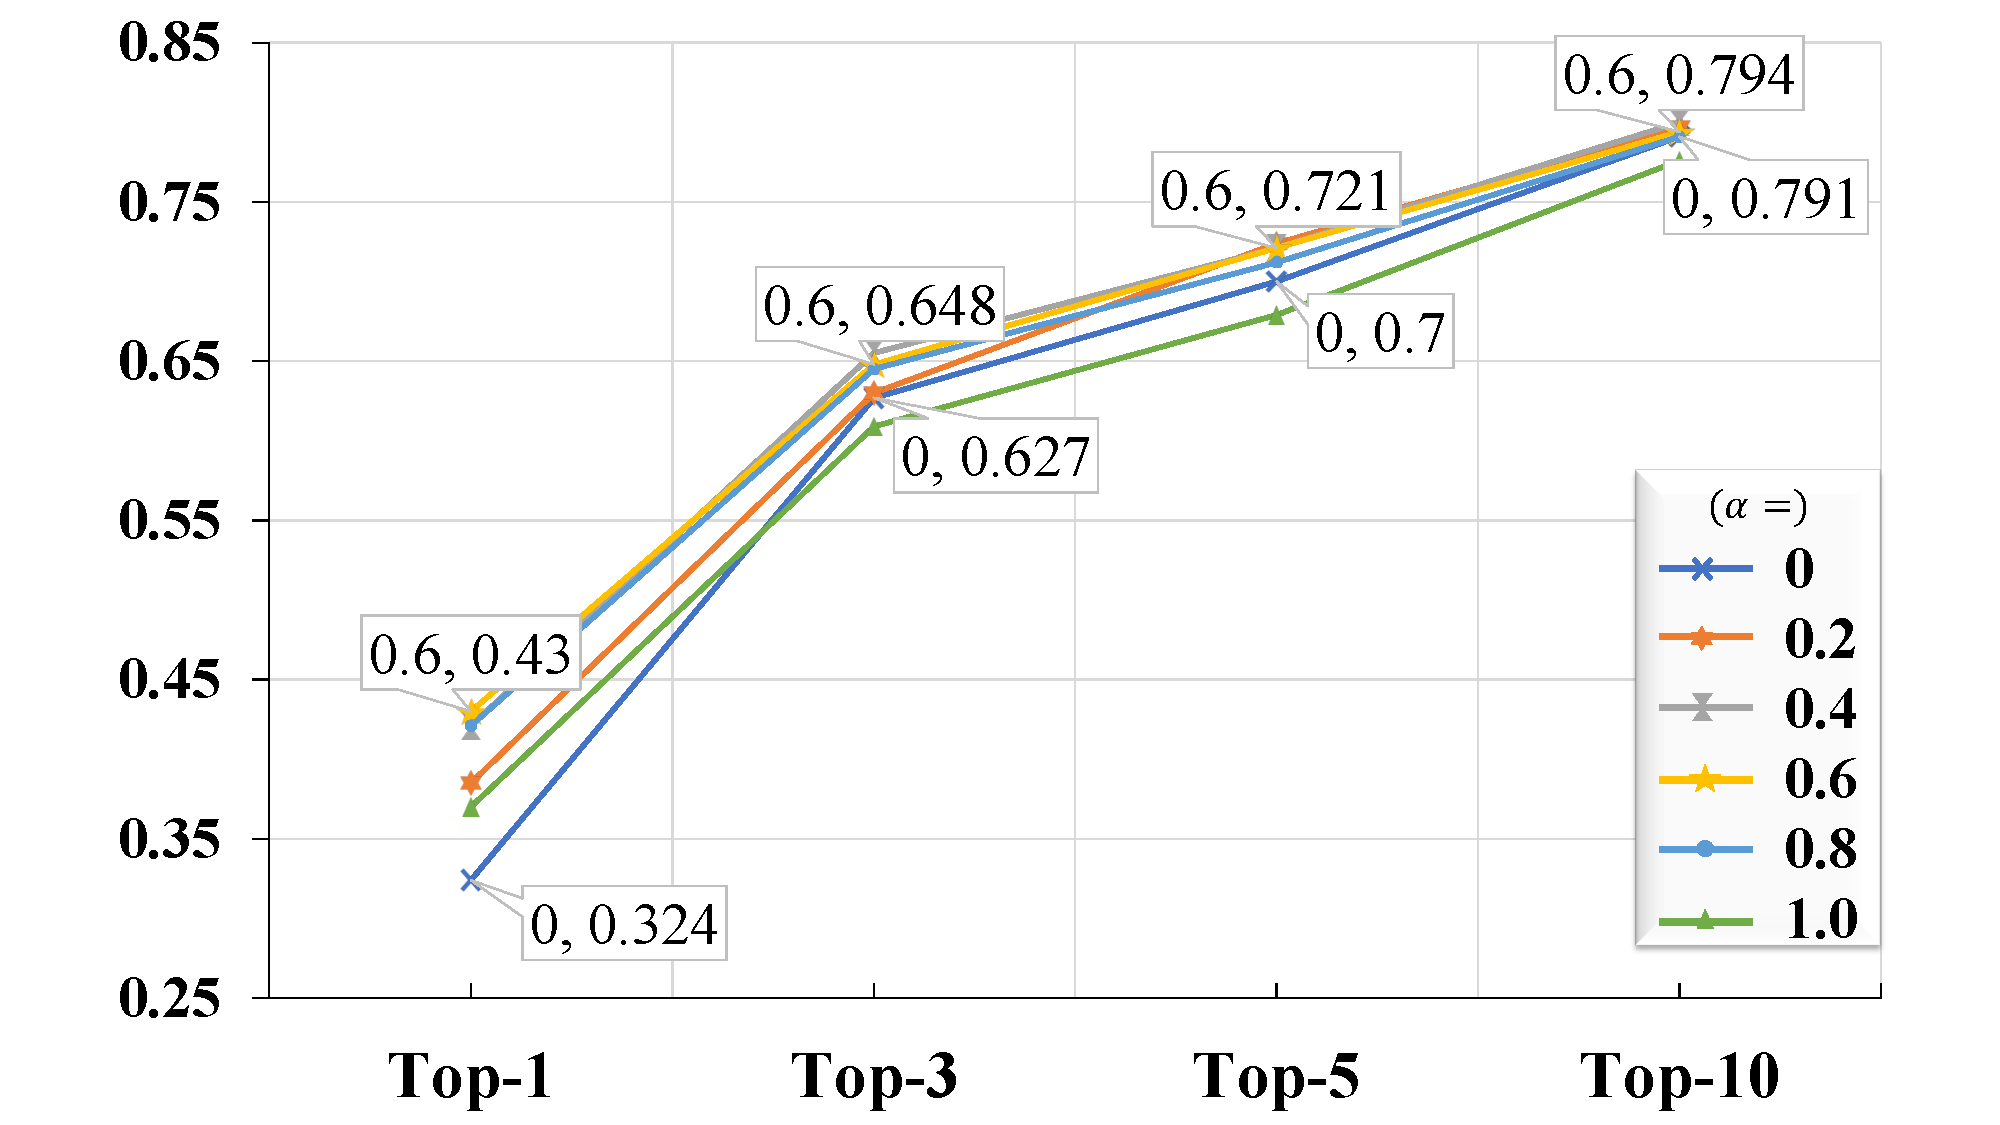
\includegraphics[width=12cm]{figure/coefficient} 
\caption{\textsc{LinPred}中$\alpha$取不同值时,其 Top-k 值的变化情况} 
\label{fig:coefficient}
\end{figure}

从图中可以看出,\textsc{LinPred}总是比原始的 SBFL 方法($\alpha = 0$)在 Top-1 上的效果好。
在 Top-k(k=3,5,10)上,\textsc{MaxPred}的效果一直垫底,
可见\textsc{MaxPred}虽然能给出比较不错的分数,但是单一的\textsc{MaxPred}无法突出缺陷的语句,需要 SBFL 和它互补。
当$\alpha$落在[0.4-0.8]之间的时候,\textsc{LinPred}的效果最好。
不过总体上来说$\alpha$值的影响不会太大。

图\ref{fig:all-figure-method-level}展示了
\textsc{MaxPred},\textsc{LinPred},基于频谱的缺陷定位和基于状态覆盖的缺陷定位
在 Defects4j 上各个项目、各个公式上 Top-1 的结果。
可以看到\textsc{LinPred}在各个项目、各个公式上都有比较好的效果。

\begin{figure}[htbp] 
\centering 
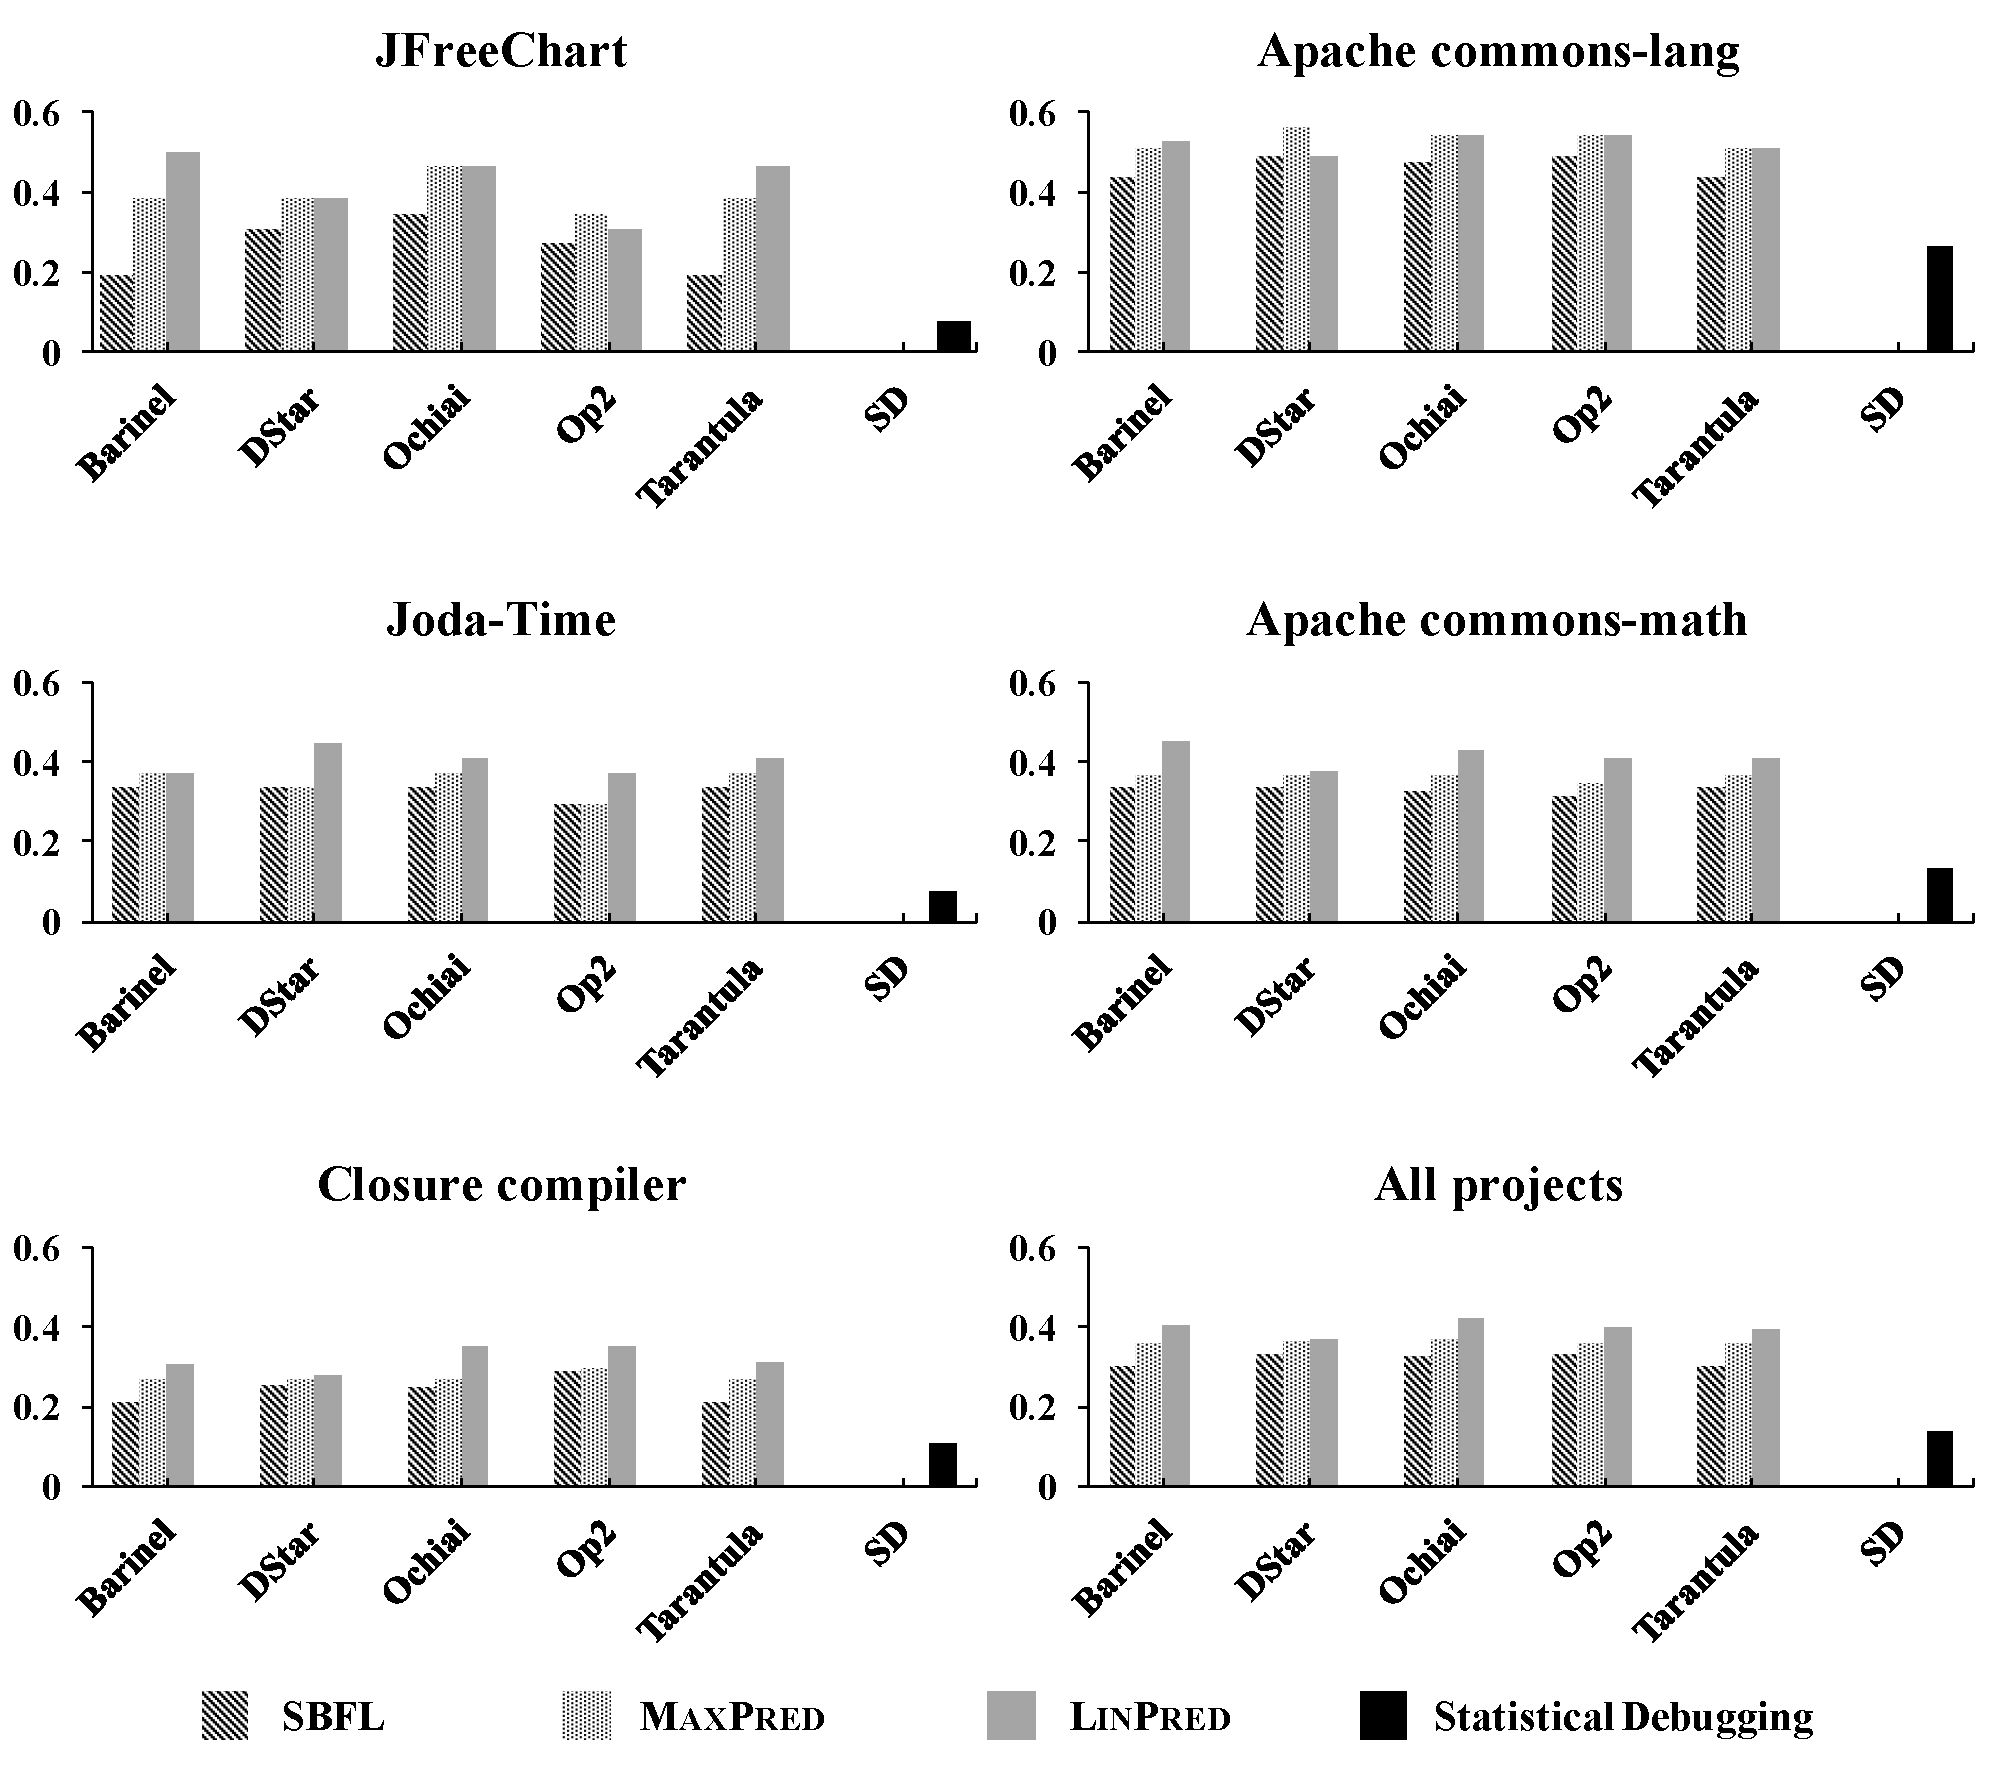
\includegraphics[width=15cm]{figure/all-figure-method-level} 
\caption{\textsc{MaxPred}、\textsc{LinPred}和传统的基于频谱和基于状态覆盖的缺陷定位在各个项目、各个公式上的 Top-1 结果对比} 
\label{fig:all-figure-method-level}
\end{figure}

\subsection{基于机器学习的谓词预测模型效果}

本小节将对基于神经网络的谓词预测模型和基于决策树的谓词预测模型的预测效果进行研究,
并回答第四个研究问题。

为了考察谓词预测模型的效果,使用验证模型,
即在章\ref{sec:gen_pred_impl}中描述的验证阶段。

先考虑VAR模型。
VAR模型的结果如表\ref{var_predict_result}所示。
整体上来看,决策树模型的准确率、查准率、查全率和F1分数都比神经网络模型的高。
所有项目的决策树模型的测试集准确率为86.71\%,
神经网络模型的为82.93\%,略低于决策树模型。
所有项目的决策树模型的测试集F1分数为86.39\%,
神经网络模型的为82.20\%。
各个项目神经网络模型的测试集准确率在79.15\%到89.00\%之间波动,
F1分数在78.10\%到88.25\%之间波动。
各个项目决策树模型的测试集准确率在85.52\%到92.81\%之间波动,
F1分数在83.63\%到92.72\%之间波动。
两个模型的结果比较接近,且效果均较好。

\begin{table}[!tbp]
\centering
\begin{tabular}{|l|l|l|l|l|l|l|l|l|}
\hline
\multirow{2}*{项目} & \multicolumn{4}{|c|}{神经网络模型} & \multicolumn{4}{|c|}{决策树模型} \\
\cline{2-9}
& 准确率 & 查准率 & 查全率 & F1分数 & 准确率 & 查准率 & 查全率 & F1分数 \\
\hline
\multirow{2}*{Math} & 85.31\% & 85.46\% & 85.31\% & 84.69\% & 89.10\% & 88.79\% & 89.10\% & 88.84\% \\
\cline{2-9}
& 89.55\% & 90.29\% & 89.55\% & 89.13\% & 97.74\% & 97.73\% & 97.74\% & 97.73\% \\
\hline
\multirow{2}*{Chart} & 89.00\% & 89.05\% & 89.00\% & 88.25\% & 92.81\% & 92.67\% & 92.81\% & 92.72\% \\
\cline{2-9}
& 90.82\% & 91.28\% & 90.82\% & 90.17\% & 97.89\% & 97.89\% & 97.89\% & 97.89\% \\
\hline
\multirow{2}*{Lang} & 83.86\% & 83.85\% & 83.86\% & 83.46\% & 85.52\% & 85.38\% & 85.52\% & 85.37\% \\
\cline{2-9}
& 90.13\% & 90.50\% & 90.13\% & 89.90\% & 96.17\% & 96.16\% & 96.17\% & 96.15\% \\
\hline
\multirow{2}*{Time} & 84.20\% & 84.30\% & 84.20\% & 83.74\% & 86.88\% & 86.80\% & 86.88\% & 86.74\% \\
\cline{2-9}
&  90.34\% & 90.84\% & 90.34\% & 90.04\% & 97.92\% & 97.92\% & 97.92\% & 97.91\% \\
\hline
\multirow{2}*{Closure} & 79.15\% & 79.12\% & 79.15\% & 78.10\% & 84.15\% & 83.52\% & 84.15\% & 83.63\% \\
\cline{2-9}
& 85.23\% & 86.31\% & 85.23\% & 84.57\% & 96.71\% & 96.69\% & 96.71\% & 96.68\% \\
\hline
\multirow{2}*{全部} & 82.93\% & 82.98\% & 82.93\% & 82.20\% & 86.71\% & 86.34\% & 86.71\% & 86.39\% \\
\cline{2-9}
& 88.20\% & 88.96\% & 88.20\% & 87.72\% & 97.09\% & 97.08\% & 97.09\% & 97.08\% \\
\hline
\end{tabular}
\caption{VAR模型的预测效果,每个项目第一行为测试集结果,第二行为训练集结果}
\label{var_predict_result}
\end{table}

再分析EXPR模型。
EXPR模型的预测结果如表\ref{expr_predict_result}。
决策树模型仍然比神经网络效果更好,且差距相比VAR模型更大。
神经网络模型的所有项目的训练集准确率都仅为38.69\%,
虽然是一个多分类问题,但是数值仍然偏低。
测试集准确率只有30.90\%。
决策树模型的所有项目的训练集准确率虽然有85.69\%,
但是测试集的准确率只有47.93\%。
EXPR模型还有很大的提升空间。

\begin{table}[!tbp]
\centering
\begin{tabular}{|l|l|l|l|l|l|l|l|l|}
\hline
\multirow{2}*{项目} & \multicolumn{4}{|c|}{神经网络模型} & \multicolumn{4}{|c|}{决策树模型} \\
\cline{2-9}
& 准确率 & 查准率 & 查全率 & F1分数 & 准确率 & 查准率 & 查全率 & F1分数 \\
\hline
\multirow{2}*{Math} & 26.01\% & 20.69\% & 26.01\% & 21.13\% & 50.51\% & 48.44\% & 50.51\% & 47.57\% \\
\cline{2-9}
& 34.19\% & 27.02\% & 34.19\% & 27.59\% & 84.07\% & 83.60\% & 84.07\% & 82.27\% \\
\hline
\multirow{2}*{Chart} & 39.42\% & 37.33\% & 39.42\% & 37.02\% & 49.44\% & 47.14\% & 49.44\% & 47.29\%\\
\cline{2-9}
& 47.48\% & 44.06\% & 47.48\% & 43.79\% & 83.49\% & 82.82\% & 83.49\% & 82.13\% \\
\hline
\multirow{2}*{Lang} & 42.67\% & 33.42\% & 42.67\% & 36.10\% & 58.93\% & 55.34\% & 58.93\% & 55.80\% \\
\cline{2-9}
& 49.92\% & 38.35\% & 49.92\% & 41.63\% & 85.76\% & 83.96\% & 85.76\% & 83.80\%\\
\hline
\multirow{2}*{Time} & 43.74\% & 33.31\% & 43.74\% & 36.87\% & 65.82\% & 62.10\% & 65.82\% & 62.63\%\\
\cline{2-9}
& 48.72\% & 36.08\% & 48.72\% & 40.14\% & 93.61\% & 92.92\% & 93.61\% & 92.66\%\\
\hline
\multirow{2}*{Closure} & 24.76\% & 19.47\% & 24.76\% & 20.98\% & 36.58\% & 32.20\% & 36.58\% & 32.98\%\\
\cline{2-9}
& 33.04\% & 25.43\% & 33.04\% & 27.40\% & 85.77\% & 85.34\% & 85.77\% & 84.35\% \\
\hline
\multirow{2}*{全部} & 30.90\% & 24.72\% & 30.90\% & 26.15\% & 47.93\% & 44.58\% & 47.93\% & 44.75\% \\
\cline{2-9}
& 38.69\% & 30.41\% & 38.69\% & 32.20\% & 85.69\% & 84.96\% & 85.69\% & 84.10\% \\
\hline
\end{tabular}
\caption{EXPR模型的预测效果,每个项目第一行为测试集结果,第二行为训练集结果}
\label{expr_predict_result}
\end{table}

然后考虑预测模型的执行时间。
这里计算的是章\ref{sec:gen_pred_impl}中验证阶段的时间,
其时间和训练阶段时间基本一致。
决策树模型的平均训练时间为23秒,
而神经网络模型的平均训练时间为1382秒,
约为23分钟。
可见神经网络的训练时间远远高于决策树模型的训练时间,
而且其准确率等指标效果不如决策树模型。

\subsection{不同谓词对结果的影响}

在之前的研究问题的分析中,我们已经发现了\textsc{LinPred}具有非常好的效果。
相比于基于频谱的缺陷定位,\textsc{LinPred}利用了谓词进行进一步的状态划分。
在本小节,我们将会深入探究谓词在缺陷定位中起的作用,来回答第五个研究问题。

谓词在项目中的平均数量如表\ref{pred_number}所示。 
Closure 因为项目较大所以谓词数量较多。

\begin{table}
\centering
\begin{tabular}{|c|c|c|c|c|c|c|}
\hline
\multirow{2}*{谓词类型} & \multicolumn{6}{|c|}{项目} \\
\cline{2-7}
~ & Chart & Lang & Time & Math & Closure & 总计 \\
\hline
预定义谓词 & 913.6 & 119.5 & 1064.2 & 1973.0 & 2426.8 & 1662.8 \\
\hline
预测谓词 & - & - & - & - & - & - \\
\hline
恒真谓词 & 566.5 & 75.8 & 892.7 & 278.3 & 3401.3 & 1470.9 \\
\hline
\end{tabular}
\caption{平均每个项目的谓词数量}
\label{pred_number}
\end{table}

\subsubsection{预定义谓词}

\begin{figure}[tbp] 
\centering 
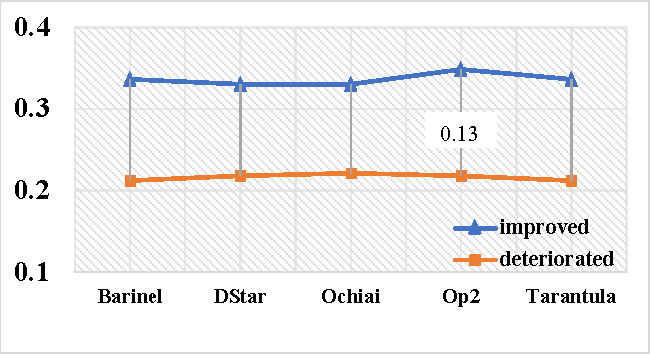
\includegraphics[width=12cm]{figure/improve-deteriorate} 
\caption{预定义谓词在缺陷定位中的作用} 
\label{fig:improve-deteriorate}
\end{figure}

首先分析谓词对定位效果的影响。
对于程序元素$e$,
一个谓词被认为是对定位效果有积极的影响,如果$c_0 > c_1$且$e$是缺陷程序元素,或者$c_0 < c_1$且$e$不是缺陷程序元素。
其中$c_0$表示使用预定义谓词的\textsc{MaxPred}的结果,
$c_1$表示基于频谱的缺陷定位的结果(谓词恒真的\textsc{MaxPred}的结果)。
一个谓词被认为是对定位效果有消极影响,如果$c_0 < c_1$且$e$是缺陷程序元素,或者$c_0 > c_1$且$e$不是缺陷程序元素。
于是谓词被分为两类,这两类在不同的怀疑度计算公式下的分布情况如图\ref{fig:improve-deteriorate}。
可以发现大部分谓词还是对结果有积极影响的,只有少部分会对结果产生不好的影响。

为了探索是三种预定义谓词中的哪种谓词起了关键作用,
我们把三种预定义谓词分别作为谓词集合,进行实验。
实验结果如图\ref{fig:diff-predictor-compare}所示。
\textsc{LinBrn}表示只使用分支谓词,
\textsc{LinRet}表示只使用返回值谓词,
\textsc{LinSca}表示只使用数值对谓词。
可以发现,\textsc{LinBrn}拥有比\textsc{LinRet}和\textsc{LinSca}更好的 Top-k(k=1,3,5,10)和 EXAM 值。
所以分支谓词的效果最明显。
\textsc{LinBrn}在 Top-1 上的效果比基于频谱的缺陷定位效果还要好,
不过基于频谱的缺陷定位在其他 Top-k 上效果更好,说明了二者的互补性。

\finding{在预定义谓词中,分支谓词对\textsc{LinPred}效果提升最明显。}

\begin{figure}[htbp] 
\centering 
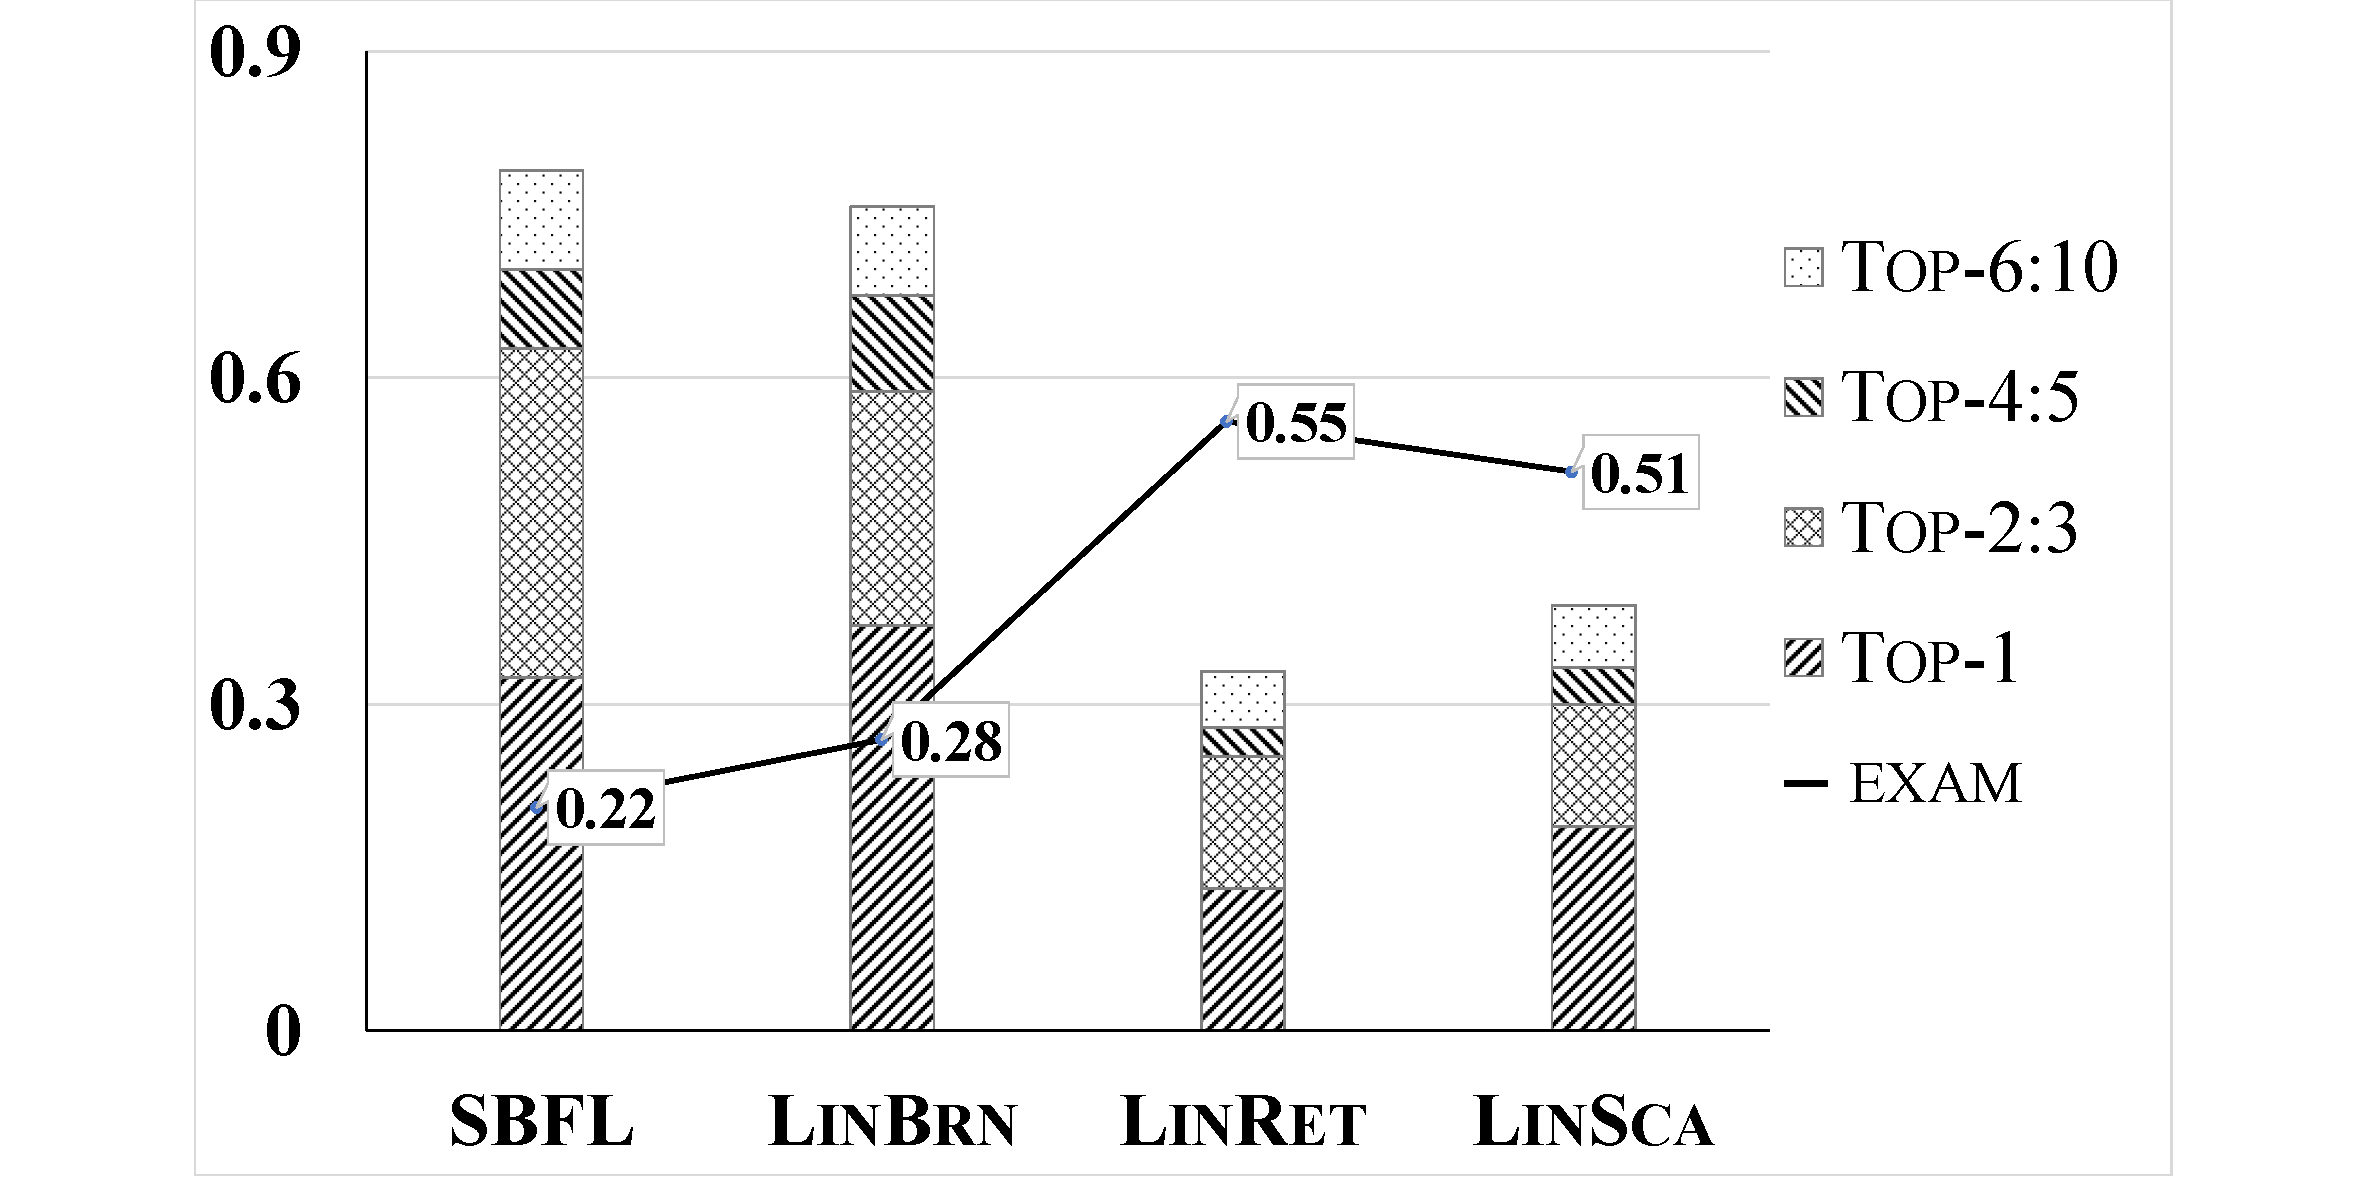
\includegraphics[width=12cm]{figure/diff-predictor-compare} 
\caption{使用不同的预定义谓词的缺陷定位效果对比} 
\label{fig:diff-predictor-compare}
\end{figure}

为了进一步验证我们的发现,我们比较了使用三种预定义谓词的\textsc{MaxPred}和
只使用了分支谓词的\textsc{MaxPred}(称为\textsc{MaxBranch}),
结果如图\ref{fig:branch-compare}。
可以发现\textsc{MaxPred}和~\textsc{MaxBranch}~的结果非常相近,
虽然\textsc{MaxBranch}少了两种谓词,但是核心的分支谓词起了很大的作用。

\begin{figure}[htbp] 
\centering 
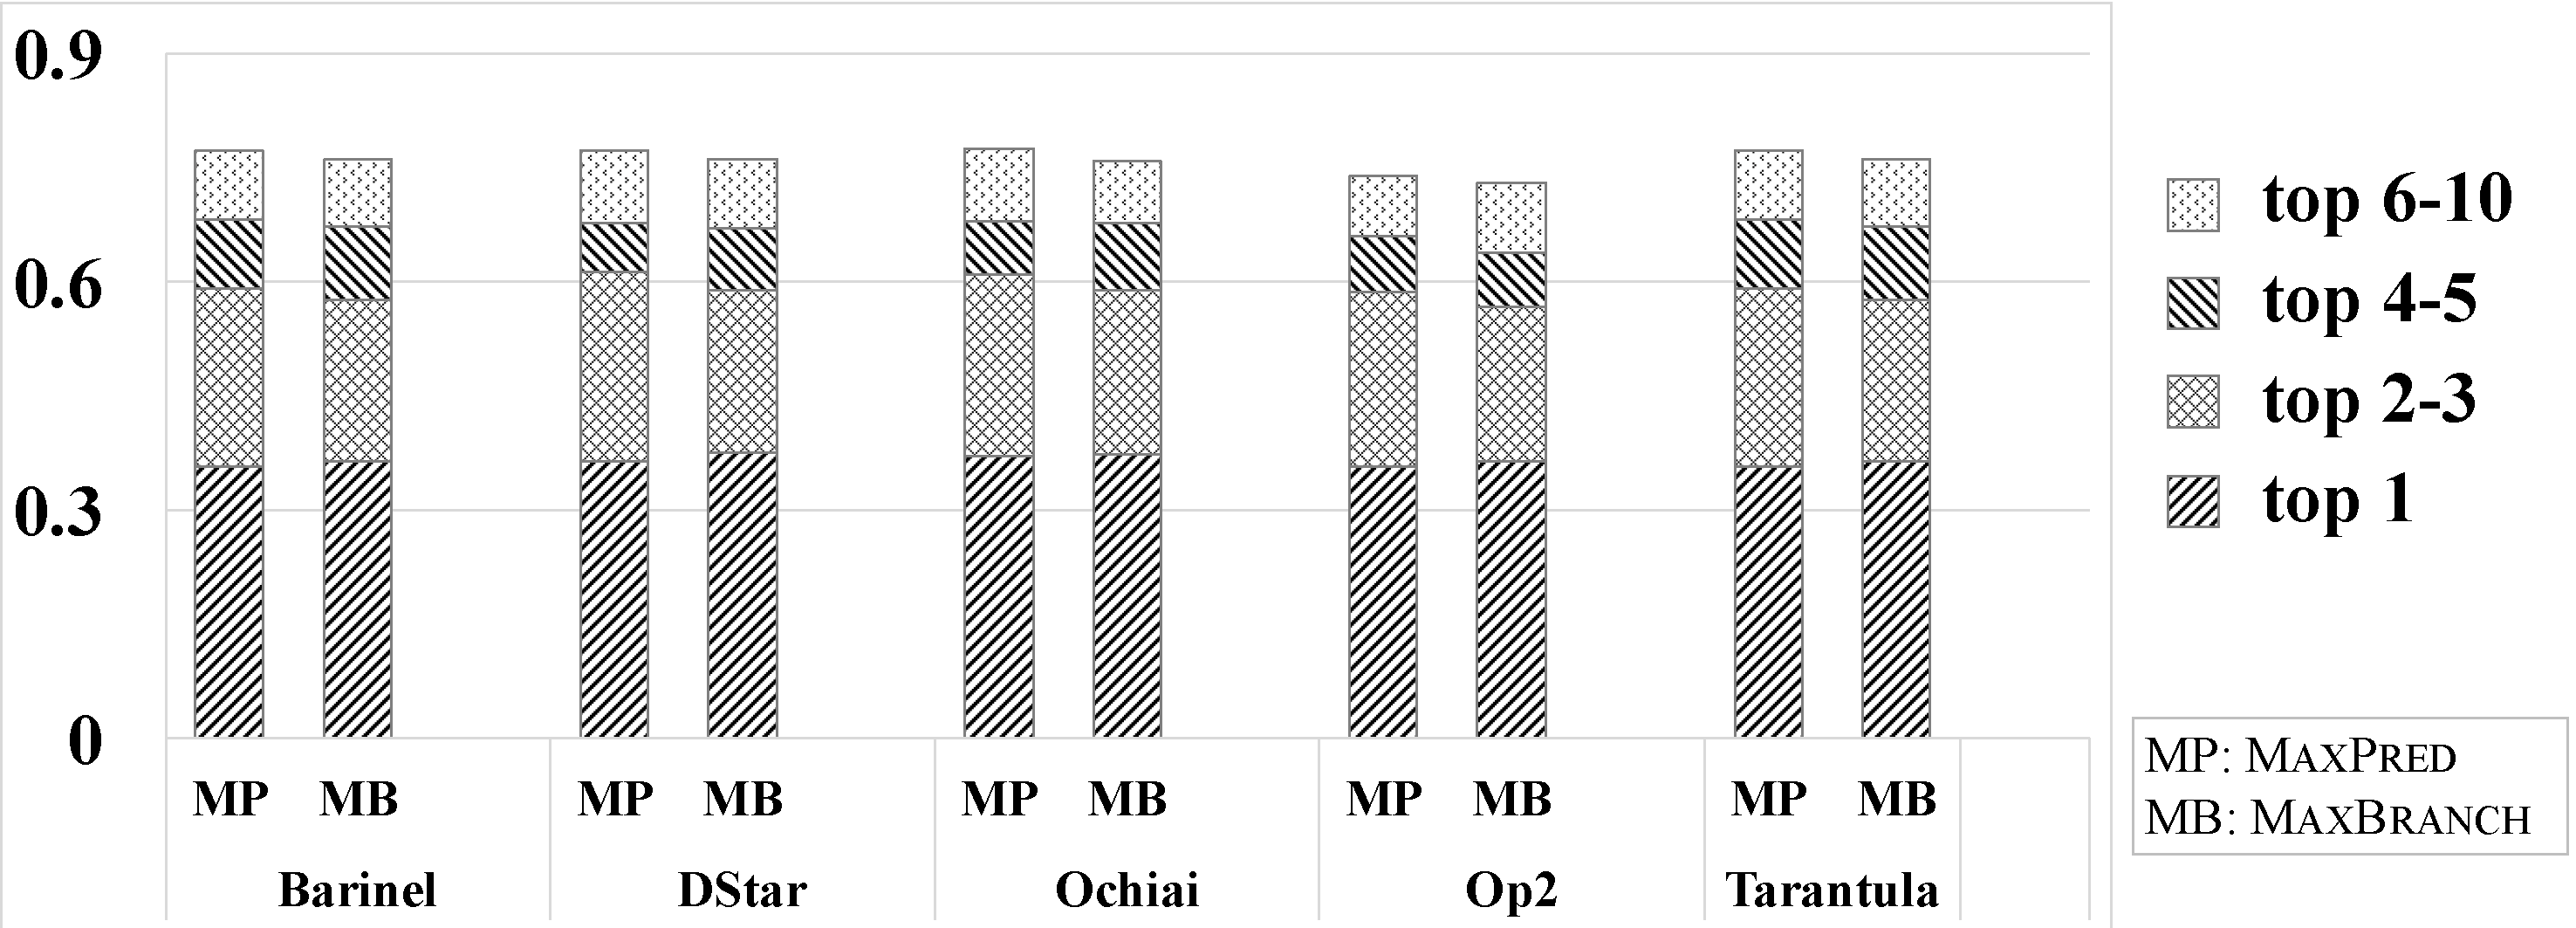
\includegraphics[width=16cm]{figure/branch-compare} 
\caption{分支谓词和全部预定义谓词的缺陷定位效果对比} 
\label{fig:branch-compare}
\end{figure}

\subsubsection{预测谓词}

把决策树模型和神经网络模型预测出的谓词,与预定义谓词和恒真谓词比较,
得到图\ref{fig:diff-ml-pred-compare}。

\textsc{LinTree}表示使用决策树模型预测的谓词,
\textsc{LinDnn}表示使用神经网络模型预测的谓词。
从Top-1和Top-3指标上看,\textsc{LinPred}的效果最好。
可见预定义的谓词在把缺陷定位在最前面具有很大优势。
而从EXAM指标上看,\textsc{LinTree}的效果最好。
虽然决策树模型预测出的谓词在把缺陷排在最前面的效果不如预定义谓词,
但是在整体上决策树模型预测出的谓词能够把缺陷排在更加考前的位置。

\todo{正负性比较}

\begin{figure}[htbp] 
\centering 
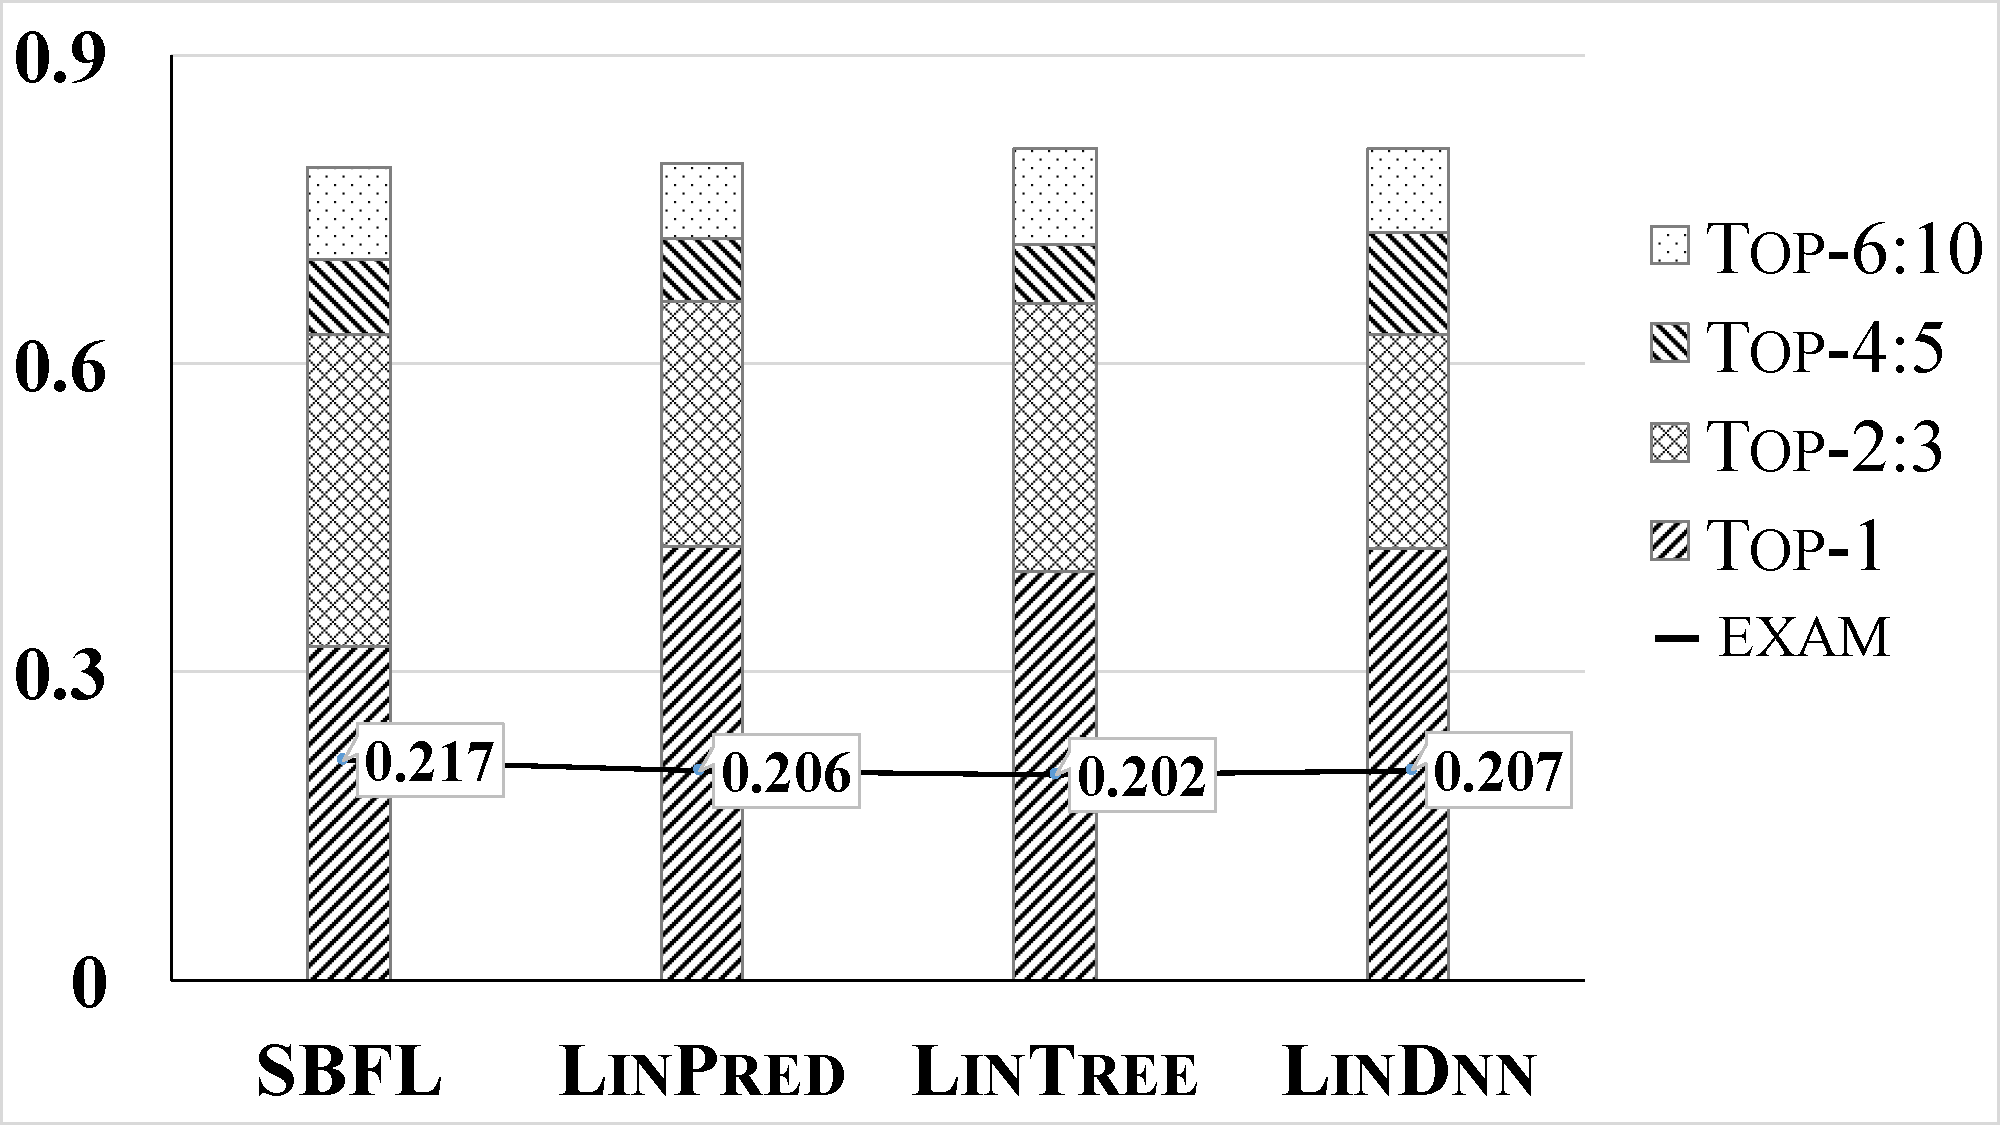
\includegraphics[width=10cm]{figure/diff-ml-pred-compare} 
\caption{预测谓词和预定义谓词的缺陷定位效果对比} 
\label{fig:diff-ml-pred-compare}
\end{figure}


	% 结论。
	% Copyright (c) 2014,2016 Casper Ti. Vector
% Public domain.

\specialchap{结论}
% \pkuthssffaq % 中文测试文字。

% vim:ts=4:sw=4


	% 正文中的附录部分。
	\appendix
	% 排版参考文献列表。bibintoc 选项使“参考文献”出现在目录中;
	% 如果同时要使参考文献列表参与章节编号,可将“bibintoc”改为“bibnumbered”。
	\printbibliography[heading = bibintoc]
	% \bibliographystyle{IEEEtran}%

	% \bibliography{thesis.bib}
	% 各附录。
	% Copyright (c) 2014,2016 Casper Ti. Vector
% Public domain.

\chapter{附件}
% \pkuthssffaq % 中文测试文字。

% vim:ts=4:sw=4


	% 以下为正文之后的部分,默认不进行章节编号。
	\backmatter
	% 致谢。
	\chapter{致谢}

感谢北京大学和北京大学软件工程所,让我能够接触到前沿的科研项目。
浓厚的学术氛围感染了我,敦促我不断学习,打下了科研的坚实基础。

感谢熊英飞研究员,张路教授和郝丹副教授对我的指导。
我从大三开始就在张路老师的小组里学习,近五年的时间里三位老师对我耐心地指导和帮助,让我受益颇多。
从最开始的浮点数计算误差相关的研究,到自动缺陷定位的研究,
我从一个初出茅庐的计算机专业低年级学生,
变成了一个能够完成很多艰难计算机任务的高年级研究生。
老师们的培养让我在计算机基础知识,代码能力,科研能力等方面都有提升。
我也在熊英飞研究和张路教授的指导下发表了两篇CCF-A类的论文,一篇第一作者,一篇第二作者。

感谢姜佳君同学,和我一起讨论、完成这个研究。
他提出了许多宝贵的想法与建议,并且与我一起实现了\textsc{LinSD}。

感谢王博同学和臧琳飞师姐,他们的基于机器学习的缺陷修复给了本文非常多的帮助。
本文使用的从Java代码中提取特征的JDT代码来自于他们的基于机器学习的缺陷修复的代码。

最后,感谢我的父母一直陪伴着我、支持着我。他们一直是我坚强的后盾。
	% 原创性声明和使用授权说明。
	% Copyright (c) 2008-2009 solvethis
% Copyright (c) 2010-2017 Casper Ti. Vector
% All rights reserved.
%
% Redistribution and use in source and binary forms, with or without
% modification, are permitted provided that the following conditions are
% met:
%
% * Redistributions of source code must retain the above copyright notice,
%   this list of conditions and the following disclaimer.
% * Redistributions in binary form must reproduce the above copyright
%   notice, this list of conditions and the following disclaimer in the
%   documentation and/or other materials provided with the distribution.
% * Neither the name of Peking University nor the names of its contributors
%   may be used to endorse or promote products derived from this software
%   without specific prior written permission.
%
% THIS SOFTWARE IS PROVIDED BY THE COPYRIGHT HOLDERS AND CONTRIBUTORS "AS
% IS" AND ANY EXPRESS OR IMPLIED WARRANTIES, INCLUDING, BUT NOT LIMITED TO,
% THE IMPLIED WARRANTIES OF MERCHANTABILITY AND FITNESS FOR A PARTICULAR
% PURPOSE ARE DISCLAIMED. IN NO EVENT SHALL THE COPYRIGHT HOLDER OR
% CONTRIBUTORS BE LIABLE FOR ANY DIRECT, INDIRECT, INCIDENTAL, SPECIAL,
% EXEMPLARY, OR CONSEQUENTIAL DAMAGES (INCLUDING, BUT NOT LIMITED TO,
% PROCUREMENT OF SUBSTITUTE GOODS OR SERVICES; LOSS OF USE, DATA, OR
% PROFITS; OR BUSINESS INTERRUPTION) HOWEVER CAUSED AND ON ANY THEORY OF
% LIABILITY, WHETHER IN CONTRACT, STRICT LIABILITY, OR TORT (INCLUDING
% NEGLIGENCE OR OTHERWISE) ARISING IN ANY WAY OUT OF THE USE OF THIS
% SOFTWARE, EVEN IF ADVISED OF THE POSSIBILITY OF SUCH DAMAGE.

{
	\ctexset{section = {
		format+ = {\centering}, beforeskip = {40bp}, afterskip = {15bp}
	}}

	% 学校书面要求本页面不要页码,但在给出的 Word 模版中又有页码且编入了目录。
	% 此处以 Word 模版为实际标准进行设定。
	\specialchap{北京大学学位论文原创性声明和使用授权说明}
	\mbox{}\vspace*{-3em}
	\section*{原创性声明}

	本人郑重声明:
	所呈交的学位论文,是本人在导师的指导下,独立进行研究工作所取得的成果。
	除文中已经注明引用的内容外,
	本论文不含任何其他个人或集体已经发表或撰写过的作品或成果。
	对本文的研究做出重要贡献的个人和集体,均已在文中以明确方式标明。
	本声明的法律结果由本人承担。
	\vskip 1em
	\rightline{%
		论文作者签名:\hspace{5em}%
		日期:\hspace{2em}年\hspace{2em}月\hspace{2em}日%
	}

	\section*{%
		学位论文使用授权说明\\[-0.33em]
		\textmd{\zihao{5}(必须装订在提交学校图书馆的印刷本)}%
	}

	本人完全了解北京大学关于收集、保存、使用学位论文的规定,即:
	\begin{itemize}
		\item 按照学校要求提交学位论文的印刷本和电子版本;
		\item 学校有权保存学位论文的印刷本和电子版,
			并提供目录检索与阅览服务,在校园网上提供服务;
		\item 学校可以采用影印、缩印、数字化或其它复制手段保存论文;
		\item 因某种特殊原因需要延迟发布学位论文电子版,
			授权学校在 $\Box$\nobreakspace{}一年 /
			$\Box$\nobreakspace{}两年 /
			$\Box$\nobreakspace{}三年以后在校园网上全文发布。
	\end{itemize}
	\centerline{(保密论文在解密后遵守此规定)}
	\vskip 1em
	\rightline{%
		论文作者签名:\hspace{5em}导师签名:\hspace{5em}%
		日期:\hspace{2em}年\hspace{2em}月\hspace{2em}日%
	}

	% 若需排版二维码,请将二维码图片重命名为“barcode”,
	% 转为合适的图片格式,并放在当前目录下,然后去掉下面 2 行的注释。
	%\vfill\noindent
	%\includegraphics[height = 5em]{barcode}
}

% vim:ts=4:sw=4

\end{document}

% vim:ts=4:sw=4
